% =============================================================================
% Project : THE_PHILOSOPHY_OF_VIABILITY
% Book    : Book I — Ontology of Viability
% Book ID : VS.B01
%
% File    : 2_MAINMATTER/PART_I_IDENTITY_AND_MANIFESTATION/
%           CHAPTER_01_IDENTITY/00_chapter_01.tex
%
% Chapter Identifier:
%   VS.B01.P01.C01
%
% Purpose:
%   Main organizational file for Chapter 01.
%   Establishes the ontological status and conceptual
%   boundaries of identity, assembles its eleven sections,
%   and summarizes the chapter's foundational conclusions
%   and unresolved questions.
%
% Assembly Policy:
%   1. Declares the chapter and its metadata.
%   2. Introduces the ontological problem of identity
%      and the scope of the chapter.
%   3. Includes the eleven authoritative section files
%      in their established order.
%   4. Concludes the chapter without introducing new
%      foundational commitments or prematurely resolving
%      questions assigned to subsequent investigations.
%
% =============================================================================


% -----------------------------------------------------------------------------
% CHAPTER DECLARATION
% -----------------------------------------------------------------------------

\chapter{Identity}
\label{ch:identity}


% -----------------------------------------------------------------------------
% CHAPTER METADATA
% -----------------------------------------------------------------------------

\def\CurrentChapterID{VS.B01.P01.C01}
\def\CurrentChapterTitle{Identity}


% -----------------------------------------------------------------------------
% CHAPTER OPENING
% -----------------------------------------------------------------------------

\begin{quote}
\textit{
The ontological inquiry into identity concerns the
determinate being of what exists: not an additional
property acquired by an already existing entity, but
an inseparable dimension of the actuality through
which an existent is the existent that it is.
}
\end{quote}


% -----------------------------------------------------------------------------
% CHAPTER INTRODUCTION
% -----------------------------------------------------------------------------

\section*{Introduction}
\addcontentsline{toc}{section}{Introduction}

Identity is a foundational problem of ontology
because an account of existence must also address
what it means for an existent to be the existent
that it is.

The question is not exhausted by distinguishing
one entity from another, describing its properties,
or establishing the conditions under which it
can be classified. It concerns the ontological
status of identity itself and its relation to
the existence of that whose identity is at issue.

The foundational commitment adopted in this
chapter is that being and identity are
ontologically inseparable, although they remain
analytically distinguishable. An existent does
not first occur as an identity-free actuality
to which identity is subsequently added.
Nor does identity constitute an independent
ontological condition that precedes the existence
of the existent.

This commitment establishes the ontological
starting point of the investigation. It does
not, by itself, provide a complete account of
the constitution of identity or determine all
the conditions under which identity is maintained
through change.

The chapter therefore examines identity through
a sequence of related but non-interchangeable
ontological questions. Following the initial
examination of the ontological problem and the
relation between being and identity, it considers
determination, unity, distinction, individuation,
numerical identity, and signature.

These investigations establish conceptual
boundaries necessary for avoiding premature
reductions. The concepts examined are relevant
to the ontological constitution and continuity
of an existent, but their precise relations to
identity cannot be settled merely by treating
any one of them as its exhaustive definition.

The principle of non-reduction developed in
the chapter consequently serves as a constraint
on ontological explanation. It prevents the
identification of identity with a single related
dimension without assuming that identity is
ontologically isolated from those dimensions.

The scope of the investigation is foundational
rather than exhaustive. It distinguishes
established commitments from provisional
constructions and unresolved questions, leaving
open matters that require further examination
within the broader ontology.

Throughout this chapter, existence and identity
are treated as independent of any knowing,
identifying, or describing subject. The inquiry
concerns the ontological status of what exists,
not the conditions under which it becomes known.

The chapter thus establishes the conceptual
and ontological foundation for the subsequent
investigation of identity and its relations
to the other dimensions of being.


% =============================================================================
% SECTION 01
% THE ONTOLOGICAL PROBLEM OF IDENTITY
% =============================================================================

% =============================================================================
% Project : THE_PHILOSOPHY_OF_VIABILITY
% Book    : Book I — Ontology of Viability
% Book ID : VS.B01
%
% File    : CHAPTER_01_IDENTITY/sections/
%           section_01_ontological_problem_of_identity.tex
%
% Section:
%   The Ontological Problem of Identity
%
% Purpose:
%   Establishes the ontological problem of identity, clarifies
%   its relation to being and determination, distinguishes
%   identity from related ontological concepts, and defines
%   the scope and limits of the present investigation.
%
% =============================================================================


\section{The Ontological Problem of Identity}
\label{sec:ontological-problem-of-identity}


% -----------------------------------------------------------------------------
% 1. THE QUESTION OF WHAT AN ENTITY IS
% -----------------------------------------------------------------------------

\subsection{The Question of What an Entity Is}

The question of identity occupies a foundational
position in ontology because it concerns what it
means for an existent to be the existent that it is.

The question is not merely how an entity differs
from other entities, how it can be characterized,
or which properties can be attributed to it.
It concerns the ontological constitution of an
existent and the status of its identity within
the actuality of its being.

To ask what an entity is therefore involves more
than establishing a list of its characteristics.
It requires examining the relation between the
entity's existence and the identity through which
it is the entity that it is.

This problem cannot be resolved by treating identity
as an additional property acquired by an entity
after its existence has already been established.
Such an approach would presuppose an entity whose
existence could be understood independently of
its being anything determinate.

Nor can identity be treated as an independent
ontological condition that precedes the existence
of the entity to which it belongs. Both approaches
separate what this investigation regards as
ontologically inseparable.

The starting point of the present inquiry is
therefore the ontological status of identity itself.
Identity must be examined as a dimension of the
actuality of what exists, rather than as a merely
descriptive characterization imposed upon it.

This formulation establishes the central problem
of the section: what is the ontological significance
of being the entity that an existent is, and how
does this identity relate to the determinations
through which its being is constituted and articulated?


% -----------------------------------------------------------------------------
% 2. IDENTITY AS AN ONTOLOGICAL PROBLEM
% -----------------------------------------------------------------------------

\subsection{Identity as an Ontological Problem Rather Than a Descriptive Problem}

Identity is frequently approached through properties,
characteristics, identifying marks, or configurations
of features. Such approaches can be useful for
characterizing entities and examining their
distinguishing features. Nevertheless, they do
not necessarily establish the ontological status
of the identity of the entities concerned.

A description may specify characteristics of
an entity without establishing whether those
characteristics are constitutive of its identity.
A distinguishing feature may differentiate one
entity from another without explaining the
ontological basis of that distinction. A
configuration of properties may characterize
an existent without exhausting what that
existent is.

The distinction between identity and its
characterization is therefore indispensable.

The identity of an entity must not be equated
with the set of statements, properties, or
descriptive features associated with it.
Such features may be relevant to its ontological
constitution, but their descriptive availability
does not establish their constitutive status.

Likewise, a characteristic may distinguish
an entity within a particular context without
being sufficient to establish its identity
in the full ontological sense.

The problem becomes more significant when
different kinds of determination are considered
together. An entity may involve structural,
relational, and material determinations. It may
participate in relations, undergo transformations,
and exhibit different manifestations. Yet the
presence of these dimensions does not, by itself,
establish how they contribute to the constitution
of its identity.

The ontological investigation must consequently
distinguish three interconnected questions:

\begin{enumerate}
    \item What is the ontological status of identity
    as a dimension of an existent?

    \item Through which determinations and relations
    is the identity of an existent constituted
    and articulated?

    \item Under what conditions can an existent
    undergo alterations in its determinations
    without necessarily losing or replacing
    its identity?
\end{enumerate}

These questions are related, but they are not
interchangeable. The first concerns the ontological
problem of identity itself. The second concerns
the relation between identity and determination.
The third introduces the problem of identity
in relation to continuity and transformation.

A satisfactory ontology of identity must preserve
these distinctions rather than treating the
description or characterization of an entity
as a sufficient explanation of its being.


% -----------------------------------------------------------------------------
% 3. THE PROBLEM OF IDENTITY AND BEING
% -----------------------------------------------------------------------------

\subsection{The Problem of Identity and Being}
\label{subsec:identity-and-being-problem}

The ontological status of identity immediately
raises the question of its relation to being.

If identity is treated as a property that an
already existing entity subsequently acquires,
the account implicitly assumes that an entity
can first exist independently of being anything
determinate.

Such an assumption creates a fundamental
ontological difficulty. An entirely identity-free
existent would lack any established basis for
being the existent that it is. The attempt to
describe what exists prior to its identity
would therefore risk presupposing the very
determination whose absence it seeks to establish.

The position developed in this work is that
being and identity are ontologically inseparable.
To exist is not to exist first as an identity-free
substrate and subsequently become an entity
through the addition of identity. Rather,
the actuality of an existent and its being
the existent that it is belong to the same
ontological actuality.

This inseparability does not eliminate the
analytical distinction between being and identity.

Being concerns the actuality of what exists,
whereas identity concerns the existent as
the existent that it is. These formulations
indicate distinguishable dimensions of one
ontological actuality; they do not establish
two independently existing components.

Three claims must nevertheless be kept distinct.

First, being and identity are analytically
distinguishable: each can be examined under
a different conceptual aspect.

Second, being and identity are ontologically
inseparable: neither is treated here as an
independently existing component that can
be detached from the other.

Third, neither is assigned ontological priority
over the other. Their analytical distinction
does not establish an order of ontological
dependence, and their inseparability does
not, by itself, demonstrate the claim of
non-priority. Non-priority is maintained
as a distinct foundational commitment.

Accordingly, the relation between being and
identity is neither one of temporal succession
nor one of external addition. Identity is not
imposed upon being, and being is not an
identity-neutral foundation that must receive
its identity from elsewhere.

This position constitutes a foundational
ontological commitment of the Viability
Philosophy System. Its implications and
conceptual limits will be examined more
precisely in Section~\ref{sec:being-and-identity}.


% -----------------------------------------------------------------------------
% 4. THE PROBLEM OF IDENTITY AND DETERMINATION
% -----------------------------------------------------------------------------

\subsection{The Problem of Identity and Determination}

The inseparability of being and identity
leads to a further question: what is the
relation between identity and determination?

An existent is not an entirely indeterminate
actuality. Its being involves a determinate
ontological character. Nevertheless, it would
be premature to conclude that every determination
associated with an existent contributes to
its identity in the same way or possesses
the same ontological status.

Some determinations may be constitutive of
the existent, whereas others may arise through
its relations, conditions, manifestations,
or participation in particular ontological
domains. Some may persist through transformations,
while others may vary or cease to obtain.

The ontological significance of these differences
cannot be assumed in advance.

The problem is therefore not simply whether
an existent is determinate, but how its
determinations relate to its identity.

This distinction prevents two opposite reductions.

On the one hand, identity cannot be separated
from determination as though an existent could
possess an actuality entirely independent of
any determinate character.

On the other hand, identity cannot be reduced
to an exhaustive inventory of all properties,
relations, or conditions associated with
an existent. The presence of a determination
does not automatically establish that it is
constitutive of identity, and the accumulation
of determinations does not, by itself,
explain their ontological unity or significance.

An adequate account must therefore investigate
which determinations are constitutive, how
they are related, and whether their alteration
is compatible with the continued identity
of the existent.

These questions will be developed in
Section~\ref{sec:identity-and-determination}.
At the present stage, it is sufficient to
establish that determination is indispensable
to the investigation of identity without
assuming that all determinations possess
the same ontological status.


% -----------------------------------------------------------------------------
% 5. THE PROBLEM OF IDENTITY AND DIFFERENCE
% -----------------------------------------------------------------------------

\subsection{The Problem of Identity and Difference}

Identity also raises the problem of difference.

To consider an existent as the existent that
it is involves distinguishing its identity
from the identity of what it is not. However,
the existence of a difference between entities
does not, by itself, explain what constitutes
the identity of either entity.

Difference and identity are therefore related
but non-equivalent ontological concerns.

A distinction may involve a particular feature,
relation, structural configuration, or material
determination. Yet the fact that a characteristic
differentiates two entities does not establish
that this characteristic constitutes the
identity of either one.

Distinguishability cannot automatically be
equated with ontological constitution.

This becomes particularly important when
considering entities that share several
determinations while remaining distinct,
as well as entities whose determinations
may vary under different conditions.

The problem of difference must therefore
be addressed without reducing identity
to the accumulation of distinguishing
properties.

The investigation will return to this issue
through the analysis of unity, distinction,
individuation, numerical identity, and
signature. At this stage, the essential
commitment is that difference may articulate
distinctions between entities without
necessarily providing a complete account
of what each entity is.


% -----------------------------------------------------------------------------
% 6. THE PROBLEM OF IDENTITY THROUGH CHANGE
% -----------------------------------------------------------------------------

\subsection{The Problem of Identity Through Change}

A further difficulty emerges when identity
is considered in relation to change.

Entities may undergo transformations in
their conditions, relations, structures,
and manifestations. Their determinations
may vary, their configurations may be
reorganized, and their relations with
other entities may be altered.

These possibilities raise a fundamental
ontological question: under what conditions
does an existent remain the existent that
it is through transformation?

The question cannot be answered simply by
asserting that identity requires the persistence
of all properties. Such a position would make
identity incompatible with any alteration
in the determinations of an existent.

Conversely, it cannot be assumed that every
existent preserves its identity regardless
of the transformations it undergoes.

Both positions require arguments that have
not yet been established.

The problem of identity through change therefore
requires an account of the relationship between
constitutive determinations and changing
conditions. It also requires distinguishing
the persistence of an existent from the
persistence of particular characteristics
associated with it.

The relation between identity and continuity
must consequently be investigated without
presupposing that continuity is equivalent
to the uninterrupted persistence of every
determination.

Likewise, the possibility of transformation
does not by itself establish either the
preservation or the replacement of identity.

The detailed examination of continuity,
persistence, and transformation requires
further conceptual and ontological analysis.
The present section establishes these issues
as problems to be investigated rather than
assuming a definitive criterion in advance.


% -----------------------------------------------------------------------------
% 7. THE DISTINCTION BETWEEN IDENTITY AND RELATED CONCEPTS
% -----------------------------------------------------------------------------

\subsection{The Distinction Between Identity and Its Related Concepts}

The ontological problem of identity cannot
be adequately formulated without distinguishing
identity from several closely related concepts.

Unity concerns the question of how an existent
constitutes a unity. It must not be assumed
that unity is equivalent to singularity,
that every unity is an aggregate, or that
unity can be explained solely through composition.

Individuation concerns the question of how
an existent is determined or distinguished
as this existent rather than another. Its
relation to identity requires independent
analysis; individuation must not simply be
substituted for identity.

Numerical identity concerns whether an existent
at different times, positions, or conditions
is one and the same existent. This question
is indispensable to the analysis of persistence
and continuity, but numerical identity alone
does not provide a complete account of the
ontological constitution of an existent.

Invariance concerns the preservation of
specified features or relations under
specified transformations and with respect
to a specified domain. It may be relevant
to the examination of identity, but the
presence of an invariant does not by itself
establish identity, and invariance is not
equivalent to persistence or continuity.

Signature concerns a structured characterization
associated with an existent. A signature may
help articulate or distinguish an existent,
but its descriptive or identifying usefulness
does not establish that it constitutes the
identity of that existent.

Determination concerns the ways in which
an existent is determinate. It is indispensable
to the inquiry into identity, but identity
cannot be equated with an exhaustive inventory
of determinations.

Expression and manifestation introduce further
questions concerning the articulation and
manifestation of ontological determinations.
Their relation to identity must be examined
without treating either concept as synonymous
with identity or presuming that either exhausts
the constitution of an existent.

These concepts are related to identity because
they address different aspects of the constitution,
differentiation, characterization, persistence,
or manifestation of existents. Nevertheless,
their relevance does not establish their
equivalence.

The principal distinctions required at this
stage are summarized in Table~\ref{tab:identity-conceptual-distinctions}.
The table provides a conceptual orientation
for the chapter; it does not claim to offer
final or exhaustive definitions of every
listed concept.

% =============================================================================
% Project : THE_PHILOSOPHY_OF_VIABILITY
% Book    : Book I — Ontology of Viability
% Book ID : VS.B01
%
% Asset   : Table
% ID      : VS.B01.P01.C01.S01.SS07.P001.TL01
% Name    : identity_conceptual_distinctions
%
% File    :
%   4_ASSETS/tables/
%   VS.B01.P01.C01.S01.SS07.P001.TL01.identity_conceptual_distinctions.tex
%
% Referenced from:
%   Chapter 01 — Section 01 — Subsection 07
%
% =============================================================================

\begin{table}[htbp]
\centering
\caption{Conceptual Distinctions Between Identity and Related Ontological Concepts}
\label{tab:identity-conceptual-distinctions}

\renewcommand{\arraystretch}{1.35}
\small

\begin{tabular}{|p{0.23\textwidth}|p{0.67\textwidth}|}
\hline
\textbf{Concept} & \textbf{Distinction from Identity} \\
\hline

Being
&
Concerns the actuality of what exists. It is
analytically distinguishable from identity but
is not treated as ontologically separable from it.
Neither is assigned ontological priority over
the other.
\\
\hline

Determination
&
Concerns the determinate character of an existent.
Determinations may be relevant to the constitution
of identity, but identity is not defined as the
sum or inventory of all determinations.
\\
\hline

Unity
&
Concerns the constitution or coherence of an
existent as a unity. Unity is not automatically
equivalent to singularity, aggregate, composition,
or identity.
\\
\hline

Individuation
&
Concerns the determination or differentiation
through which an existent is distinguished as
this existent. Its relation to identity requires
analysis and cannot be assumed to be equivalent
to identity.
\\
\hline

Numerical Identity
&
Concerns whether an existent considered across
different times, positions, or conditions is
one and the same existent. This question does
not, by itself, exhaust the ontological constitution
of that existent.
\\
\hline

Difference
&
Concerns distinction or non-identity between
entities or determinations. A difference may
distinguish entities without necessarily
establishing what constitutes the identity
of either one.
\\
\hline

Invariance
&
Concerns the preservation of specified features
or relations under specified transformations
and with respect to a specified domain. An
invariant does not, by itself, establish
identity, persistence, or continuity.
\\
\hline

Signature
&
Concerns a structured characterization associated
with an existent. A signature may contribute
to its characterization or differentiation
without necessarily constituting its identity.
\\
\hline

Expression
&
Concerns the articulation of determinations
or aspects of an existent. It must not be
treated as synonymous with identity or as
an exhaustive account of its constitution.
\\
\hline

Manifestation
&
Concerns how an existent or its determinations
are manifested. A manifestation is not,
without further argument, identical to the
identity of that which is manifested.
\\
\hline

Continuity
&
Concerns a relation of connectedness or
continuation across conditions or stages.
It must not be equated in advance with
identity preservation or with the persistence
of every determination.
\\
\hline

\end{tabular}

\end{table}

% =============================================================================
% END OF TABLE
% =============================================================================

The distinctions in Table~\ref{tab:identity-conceptual-distinctions}
are not intended to establish a complete theory
of every listed concept.

Their purpose is to prevent conceptual substitution:
a concept related to identity must not be treated
as identical to identity without an independent
ontological argument.

Nor should conceptual distinction be interpreted
as proof of ontological independence. The fact
that two concepts can be analytically distinguished
does not establish that the corresponding
ontological dimensions exist independently
of one another.


% -----------------------------------------------------------------------------
% 8. THE SCOPE OF THE ONTOLOGICAL INVESTIGATION
% -----------------------------------------------------------------------------

\subsection{The Scope of the Ontological Investigation}

The scope of the present investigation
must be clearly delimited.

First, identity is examined as an ontological
dimension of what exists. Its existence
and constitution are not made dependent upon
the presence or activity of an external
identifying subject.

Second, the investigation does not assume
that the identity of an existent can be
exhaustively captured through a set of
properties or distinguishing characteristics.
Such characteristics may be relevant to
its constitution, but their constitutive
significance must be established rather
than presumed.

Third, the investigation does not assume
that an existent necessarily possesses
only one identity. The possibility of
multiple identities within one existent,
including the possibility that different
respects or ontological levels may be relevant
to different aspects of identity, remains
an open question. Neither a plurality of
manifestations nor a plurality of components
is, by itself, evidence of a plurality
of identities.

Fourth, the investigation does not equate
identity preservation with the persistence
of all properties or the absence of change.
The relationship between identity and
transformation requires an account of
constitutive determinations and the
conditions under which their alteration
may be compatible with identity.

Fifth, the investigation does not assume
that identity is reducible to composition,
structure, relation, materiality, or
manifestation. These dimensions may be
relevant to the ontological constitution
of an existent, but their precise roles
must be established through the subsequent
development of the ontology.

Finally, the present section does not
attempt to provide a complete account
of the organization of the realms of being,
the ontological status of light, or the
dynamics through which determinations
are articulated and transformed.

These questions require the development
of the subsequent investigations within
the architecture of the Ontology of Viability.

These limitations are not arbitrary restrictions.
They preserve the distinction between the
foundational problem of identity and the
additional ontological questions required
for its more comprehensive explanation.


% -----------------------------------------------------------------------------
% 9. THE CENTRAL ONTOLOGICAL PROBLEM
% -----------------------------------------------------------------------------

\subsection{The Central Ontological Problem}

The preceding considerations allow the
central problem of this section to be
formulated more precisely.

The question is not merely how an existent
can be distinguished from other existents,
or how its characteristics can be described.
The question is what constitutes an existent
as the existent that it is, how this identity
belongs to its ontological actuality, and
how it relates to the determinations and
transformations through which its being
is articulated.

This problem contains several interconnected
dimensions:

\begin{enumerate}
    \item The analytical distinction and
    ontological inseparability of being
    and identity, together with the distinct
    commitment that neither has ontological
    priority over the other.

    \item The relation between identity
    and the determinations that may be
    constitutive of an existent.

    \item The distinction between identity,
    unity, distinction, and individuation.

    \item The relation between identity
    and difference.

    \item The distinction between identity
    and its descriptive or characterizing
    dimensions, particularly signature.

    \item The relationship between identity,
    numerical identity, continuity, and
    transformation.

    \item The possibility of plurality
    of identities within a single existent,
    without presupposing either unity or
    plurality as the necessary outcome.
\end{enumerate}

These dimensions cannot be resolved through
a single definition or by reducing identity
to one of its associated concepts.

They require a systematic ontological
investigation in which the relations among
them are established without prematurely
collapsing their distinctions.

The purpose of this chapter is therefore
to establish the conceptual and ontological
foundations necessary for such an investigation.
It begins with the inseparability of being
and identity, proceeds to the relationship
between identity and determination, examines
unity, distinction, and individuation, and
subsequently investigates numerical identity,
signature, and the principle of non-reduction.

The chapter does not presume that all these
relations have already been resolved. Rather,
it establishes the problem-space within which
their ontological significance can be
rigorously examined.


% -----------------------------------------------------------------------------
% 10. CONCLUDING FORMULATION
% -----------------------------------------------------------------------------

\subsection{Concluding Formulation}

Identity is not an additional property of
an existent, nor is it merely a descriptive
representation of its characteristics or
a criterion through which it can be
distinguished from other existents.

It is an ontological concern inseparable
from the actuality of being.

To investigate identity is therefore to
investigate what it means for an existent
to be the existent that it is, how this
identity belongs to its ontological
constitution, and how it relates to the
plurality of determinations, relations,
and transformations through which its
being is articulated.

The central position established here
distinguishes three claims: being and
identity are analytically distinguishable;
they are ontologically inseparable; and
neither is assigned ontological priority
over the other. These claims are related,
but none is treated as an automatic
demonstration of either of the others.

This position provides the foundation
for the subsequent examination of identity.
It also establishes a necessary restriction:
no related concept may replace identity
without an independent ontological argument,
and no analytical distinction may be taken
as sufficient proof of ontological independence.

The ontological problem of identity is thus
established as the starting point for the
systematic investigation undertaken in
the following sections.


% =============================================================================
% END OF SECTION
% =============================================================================


% =============================================================================
% SECTION 02
% BEING AND IDENTITY
% =============================================================================


\section{Being and Identity}
\label{sec:being-and-identity}

\subsection{The Ontological Inseparability of Being and Identity}

The relation between being and identity constitutes one of the
foundational problems of ontology. Any account of what it means for
something to be must also address what makes that existent the existent
that it is. Being cannot be adequately considered without addressing
identity, just as identity cannot be understood independently of the
being whose identity it is.

The position developed here begins with a fundamental proposition:
being and identity are ontologically inseparable. They do not constitute
two independently established realities that subsequently enter into a
relationship. Nor does identity arise as an additional property
attributed to an entity that already exists in a fully constituted
ontological condition.

To say that something exists is, in this framework, to acknowledge
that it is determinate as the existent that it is. Its identity is not
an external qualification imposed upon its existence. It belongs to
the ontological actuality of that existence.

This proposition does not mean that the concepts of being and identity
are synonymous. Their conceptual distinction remains necessary.
Being concerns the actuality of existence, whereas identity concerns
the ontological self-determination through which an existent is the
existent that it is. These formulations identify analytically
distinguishable dimensions of an inseparable ontological actuality.

The distinction is therefore analytical rather than ontologically
separative. It allows the relation between existence and its
determinate character to be examined without converting them into
independent ontological components.

\subsection{Against the Priority of an Indeterminate Existent}

A possible account of existence assumes that an entity first exists
and subsequently acquires an identity through the addition of
properties, characteristics, or determinations. According to this
account, existence is initially considered independently of identity,
while identity is treated as a secondary condition that makes an
already existing entity identifiable or distinguishable.

The present ontology does not adopt this position.

An existent entirely devoid of identity would not constitute a
meaningful ontological starting point. If nothing could be said about
what makes an existent the existent that it is, then the supposed
existent would have been abstracted from the very condition through
which its existence is determinate.

This does not imply that every existent must possess a fully
articulated, externally accessible, or exhaustively describable
configuration. It means that the absence of a complete description
cannot be equated with the absence of identity.

The distinction is important. Ontological determination does not
depend upon whether an entity can be comprehensively characterized.
The limitations of a description do not establish a corresponding
indeterminacy in the existent itself.

Consequently, the distinction between an existent and its description
must not be confused with a distinction between existence and identity.
The former is legitimate; the latter, when interpreted as an
ontological separation, is rejected here.

\subsection{Being as Ontological Actuality}

Being is approached in this ontology as the actuality of existence,
rather than as a descriptive category, a linguistic designation, or
an abstraction constructed through conceptual operations.

An existent is not made real by being named, represented, classified,
or recognized. Its ontological actuality is not dependent upon the
presence of an entity capable of apprehending it.

This independence is essential to the scope of the present
investigation. The ontology of viability must establish its account
of existence without presupposing a knowing subject or making
existence conditional upon epistemic accessibility.

The fact that an existent may be unknown, incompletely described,
or inaccessible within a particular domain does not by itself
diminish its ontological actuality. Such limitations concern the
conditions under which an existent may become accessible within a
particular relation or domain. They do not constitute the ground of
its being.

Being must therefore be distinguished from the ways in which an
existent may be expressed, manifested, differentiated, or described.
These relations may be ontologically significant, but none can be
identified with existence as such without further argument.

The present section does not attempt to provide an exhaustive
definition of being. Its immediate purpose is more restricted:
to establish that being cannot be treated as an identity-free
ontological substrate.

\subsection{Identity as the Determinate Character of Being}

If being and identity are inseparable, the question arises as to
what identity contributes to the ontological constitution of an
existent.

Identity is not understood here as a list of properties, a collection
of observable features, or a descriptive profile. Such accounts may
characterize aspects of an existent, but they do not necessarily
establish what makes that existent the existent that it is.

Identity concerns the determinate character of existence itself.
It expresses the fact that an existent is not merely an unspecified
possibility but is ontologically constituted as something determinate.

This formulation must not be interpreted as reducing identity to
determination in its most general sense. Not every determination
necessarily constitutes identity, and not every feature associated
with an existent has the same ontological significance.

The distinction between constitutive determination and other forms
of determination requires a separate analysis. At this stage, the
essential claim is that identity cannot be detached from the
determinate actuality of being.

Identity is therefore neither an additional object within an entity
nor a separate entity standing alongside it. It is an ontological
dimension of the existent's own actuality.

\subsection{The Distinction Between Ontological Inseparability and Conceptual Identity}

The inseparability of being and identity does not eliminate the
possibility of distinguishing them conceptually.

Several ontological concepts may refer to dimensions of the same
existent without being interchangeable. The existence of an entity,
its identity, its unity, its individuation, and its particular
determinations may be examined separately while remaining related
within the same ontological actuality.

The distinction between conceptual differentiation and ontological
separation is therefore indispensable.

Conceptual differentiation makes it possible to investigate
different questions:

\begin{itemize}
    \item Being concerns the actuality of an existent.
    \item Identity concerns what makes that existent the existent
    that it is.
    \item Determination concerns the ways in which an existent is
    constituted as determinate.
    \item Unity concerns the ontological coherence of an existent.
    \item Individuation concerns its constitution as a distinct
    existent.
\end{itemize}

These questions are related, but their answers cannot be presumed
to be identical. In particular, the inseparability of being and
identity does not establish that identity is equivalent to unity,
individuation, or any particular form of determination.

The analytical distinction also prevents the opposite error:
treating every conceptually distinguishable dimension as an
independent ontological component.

The ontology developed in this work therefore distinguishes
without fragmenting and relates without collapsing.

\subsection{Identity and the Problem of an Underlying Substrate}

A further difficulty emerges when being is conceived as an
indeterminate substrate that remains ontologically prior to all
determinations.

Under this interpretation, identity may appear to be something
that happens to an underlying existent, rather than something
inseparable from the actuality of that existent.

The difficulty is not merely terminological. It concerns the
ontological status attributed to the supposedly underlying substrate.

If the substrate exists independently of every determination,
then the account must explain what makes it an existent rather
than an abstract possibility. If it possesses no identity whatsoever,
its status as a particular existent remains unexplained.

This ontology does not deny that abstraction may distinguish
existence from particular determinations for analytical purposes.
It rejects the further conclusion that such abstraction reveals
an independently existing, identity-free reality.

An analytical abstraction cannot, by itself, establish the
ontological independence of what it abstracts.

Accordingly, the concept of an underlying substrate must not be
used to reintroduce an ontological priority of being over identity
without an independent argument establishing that priority.

The present position is not that every question concerning
ontological grounds has already been resolved. Rather, it establishes
a constraint on subsequent explanations: no account may assume
an identity-free existent as its starting point without explaining
how such an existent could be ontologically actual.

\subsection{Being, Identity, and the Possibility of Difference}

The inseparability of being and identity also has implications
for the problem of difference.

If an existent is ontologically determinate, it cannot be considered
in complete abstraction from the conditions through which it is
distinct from other existents or from other possible configurations
of existence.

Nevertheless, identity must not be reduced to difference.
Difference concerns a relation or distinction, whereas identity
concerns the determinate actuality of the existent itself.

An entity may be distinguished from another without its identity
being exhausted by that distinction. Likewise, the fact that
different entities share certain determinations does not establish
that they possess the same identity.

The ontological relation between identity and difference therefore
requires an account that preserves both determination and
distinction without making either one reducible to the other.

This issue will be examined more extensively in the subsequent
analysis of identity and distinction.

\subsection{The Independence of Being and Identity from the Knowing Subject}

The ontological relation between being and identity must be
established independently of the conditions of knowledge.

An existent does not acquire being through recognition, nor does
its identity originate in the act of identifying it. The existence
of a knowing subject may introduce particular relations to an
existent, but such relations do not constitute the necessary
foundation of the existent's being or identity.

This position excludes an epistemic criterion from the foundational
definition of identity. An entity does not need to be known,
recognized, represented, or successfully distinguished by a
subject in order to possess identity.

It also excludes the assumption that the limits of knowledge
determine the limits of being. An existent may exceed any particular
description without thereby becoming ontologically indeterminate.

The present ontology consequently treats the knowing subject
as unnecessary to the establishment of the being--identity relation.
The analysis of how a knowing entity can apprehend existence,
including the conditions and limitations of such apprehension,
belongs to a distinct epistemological investigation.

This methodological boundary is not a denial of the reality of
knowledge. It is a distinction between the ontological constitution
of what exists and the epistemological conditions under which
existence may become known.

\subsection{Ontological Consequences of the Being--Identity Relation}

The inseparability of being and identity establishes several
constraints for the ontology of viability.

First, existence cannot be defined as an identity-free actuality
to which identity is subsequently added.

Second, identity cannot be treated as an external property,
descriptive label, or epistemic construction whose presence
depends upon recognition.

Third, conceptual distinctions between being, identity,
determination, unity, individuation, and difference must be
preserved without assuming that each distinction corresponds
to an independently existing ontological component.

Fourth, the incompleteness of a description must not be confused
with the absence or incompleteness of the existent's ontological
identity.

Fifth, no particular descriptive configuration, manifestation,
or invariant can be assumed to exhaust identity merely because
it provides a means of distinguishing or characterizing an existent.

These consequences do not yet provide a complete theory of
identity. They establish the ontological conditions within which
such a theory must be developed.

In particular, the relation between identity and constitutive
determination, the relation between identity and unity, and the
possibility of multiple identities associated with a single existent
remain questions requiring further examination.

\subsection{Concluding Formulation}

Being and identity are neither two independent ontological
realities nor two interchangeable concepts. They are analytically
distinguishable dimensions of an inseparable ontological actuality.

Being refers to the actuality of existence; identity refers to
the determinate character through which an existent is the existent
that it is. Neither has ontological priority over the other.
Identity is not subsequently added to being, and being is not
an identity-free substrate awaiting determination.

This position establishes a foundational principle for the
ontology of viability:

\begin{quote}
An existent does not first exist and then acquire an identity.
Its existence and its being-the-existent-that-it-is are
ontologically inseparable, although they remain conceptually
distinguishable.
\end{quote}

This principle does not resolve every question concerning the
constitution, unity, individuation, persistence, or multiplicity
of identity. It establishes the ontological ground from which
those questions must be investigated.

The subsequent analysis will therefore examine how identity
relates to determination, without presuming that the general
inseparability of being and identity has already settled the
specific structure of their constitutive relation.



% =============================================================================
% SECTION 03
% IDENTITY AND DETERMINATION
% =============================================================================


\section{Identity and Determination}
\label{sec:identity-and-determination}

\subsection{The Ontological Problem of Determination}

The relation between identity and determination is fundamental to
understanding how an existent is the existent that it is. If being
and identity are ontologically inseparable, as established in the
preceding section, then the determinate character of an existent
cannot be treated as an accidental addition to an otherwise
complete and identity-free existence.

Yet this proposition raises a further question: what is the
relationship between identity and determination? Are they
different expressions of the same ontological condition, or
does determination constitute a broader field within which
identity is established?

The present analysis adopts a distinction between the general
condition of being determinate and the particular determinations
that contribute to the constitution of an existent's identity.

An existent is not an indeterminate actuality to which all
determinations are subsequently attached. Its existence is
already identity-bearing. Nevertheless, this does not imply
that every determination associated with it is constitutive
of its identity.

The distinction is essential. Without it, identity would become
indistinguishable from the totality of an entity's properties,
relations, states, and characteristics. Such an identification
would make identity excessively dependent upon every variation
in the existent and would eliminate the possibility of
distinguishing constitutive conditions from non-constitutive ones.

The problem, therefore, is not simply whether identity requires
determination. It is how determination relates to identity,
which determinations participate in its constitution, and
whether different determinations possess different ontological
roles.

\subsection{Determination as an Ontological Condition}

Determination concerns the fact that an existent is not merely
an unspecified possibility. It is constituted in a determinate
manner.

This formulation does not imply that determination must always
take the form of an externally observable property or an
independently identifiable feature. Nor does it imply that
every determination must be accessible through a particular
mode of manifestation.

Determination is considered here as an ontological condition
rather than merely a descriptive operation.

An existent may possess determinations that are not directly
manifested, not externally distinguishable, or not included
in any particular description. Their lack of accessibility
does not, by itself, establish their ontological absence.

It is therefore necessary to distinguish between determination
and the description of determination. The former concerns
the ontological constitution of an existent; the latter concerns
a representation or characterization of some aspect of that
constitution.

This distinction also prevents the reduction of determination
to classification. Assigning a category to an existent does
not necessarily establish the ontological conditions through
which it is determinate.

Determination must consequently be examined in relation to
the existent itself, rather than being defined exclusively
through the operations by which it may be described.

\subsection{Identity and the Constitutive Role of Determination}

Identity cannot be separated from the determinate actuality
of an existent. However, the relationship between identity
and determination requires more precision than the general
claim that identity involves determination.

Not every determination is necessarily constitutive of identity.
An existent may undergo changes in state, acquire or lose
particular relations, or exhibit different characteristics
without thereby becoming an entirely different existent.

If every determination were automatically identity-constitutive,
any change in any property or relation would necessarily entail
a change of identity. Such a conclusion cannot be assumed.

The present framework therefore distinguishes between
determinations that participate in constituting an existent's
identity and determinations that characterize other aspects
of its actuality.

A constitutive determination is not simply a feature that
happens to be associated with an entity. It contributes to
the ontological constitution through which that entity is
the entity that it is.

This does not yet provide a complete criterion for identifying
all constitutive determinations. Establishing such a criterion
requires further investigation into the structure of identity,
the conditions of persistence, and the relation between
determination and change.

At this stage, the distinction establishes a necessary
constraint: identity cannot be reduced to the aggregate of
all determinations, and the constitutive significance of
any particular determination must be demonstrated rather
than presumed.

\subsection{Internal and Relational Determination}

Determinations may be considered in terms of their different
ontological relations to an existent.

One important distinction concerns internal and relational
determination.

Internal determination refers to a determination considered
in relation to the constitution of the existent itself.
It concerns aspects of how the existent is constituted,
rather than merely how it is positioned in relation to
something else.

Relational determination concerns determinations that arise
through, or are constituted within, relations involving
the existent and other entities, conditions, or domains.

This distinction should not be interpreted as establishing
two completely independent classes of reality. An existent
may possess an internal constitution that is inseparable
from certain relations, and relational determinations may
have consequences for its internal constitution.

Nor should internal determination automatically be identified
with identity and relational determination with non-identity.
Such an identification would prematurely establish that
identity is exclusively intrinsic and that relations are
ontologically external to it.

The possibility that certain relations may be constitutive
of an existent's identity must remain open to investigation.

The relevant question is not whether a determination is
internal or relational in isolation, but what ontological
role it performs in the constitution of the existent.

\subsection{Structural Determination}

Structural determination concerns the organization and
configuration of determinations within an existent.

An existent may involve multiple determinations that are
not merely present as an unordered collection. Their
organization, interdependence, and relations may contribute
to the way in which the existent is constituted.

Structure must therefore be distinguished from the mere
aggregate of properties.

A collection of determinations does not necessarily constitute
a coherent structure. Structural determination involves
relations among determinations and the organization through
which they participate in a more comprehensive configuration.

The significance of structure for identity cannot, however,
be settled by assuming that every structural feature is
identity-constitutive.

Some structural arrangements may be essential to the identity
of an existent, while others may admit variation without
necessarily altering that identity. Determining which
arrangements are constitutive requires an account of the
specific ontological organization under consideration.

It is also necessary to avoid identifying structure with
signature. A structural configuration may contribute to
the characterization of an existent, but a description
of that configuration does not necessarily exhaust the
existent's identity.

The distinction between structural determination and
descriptive characterization will therefore remain important
throughout the subsequent analysis.

\subsection{Material Determination}

Material determination concerns determinations associated
with the material constitution of an existent.

Material constitution may contribute to the identity of
an existent in ways that cannot be reduced to a list of
observable material properties. The ontological significance
of material determinations depends upon the kind of existent
and the role that such determinations perform in its constitution.

It would therefore be premature to claim either that material
determinations always constitute identity or that they are
merely external conditions of its manifestation.

An existent may undergo material variation while retaining
some form of identity. Conversely, particular material
determinations may be indispensable to the identity of
certain existents.

These possibilities indicate that the relation between
material determination and identity cannot be resolved
through a universal assumption that every material change
either preserves or destroys identity.

The relevant conditions must be investigated in relation
to the ontological constitution of the existent and the
specific kind of identity under consideration.

Material determination is thus recognized as an ontologically
significant domain of inquiry, without being elevated into
a universal and exhaustive definition of identity.

\subsection{Determination and Distinction}

Determination is closely related to distinction, but the
two concepts must not be conflated.

To be determinate is to possess a specific ontological
constitution. To be distinct is to stand in a condition
of difference or non-identity in relation to something
else.

Determination may provide conditions through which an
existent is distinguishable, but distinguishability does
not necessarily exhaust its identity.

Two existents may share many determinations without becoming
numerically identical. Likewise, a particular existent
may possess determinations that do not distinguish it
from every other existent.

Consequently, the relationship between identity and
determination cannot be reduced to the capacity of a
description to differentiate one entity from another.

An account of identity must address the ontological
constitution of the existent itself, rather than merely
the conditions under which it can be distinguished.

This distinction also prevents the assumption that
uniqueness of a descriptive configuration is sufficient
to establish identity. A distinctive configuration may
provide evidence of difference, but its ontological
significance must be separately established.

\subsection{Determination and Change}

The relationship between determination and change presents
a particularly important problem.

An existent may undergo changes in some of its determinations
without necessarily losing its identity. If determination
were equivalent to identity in an undifferentiated sense,
every alteration would imply a corresponding identity
replacement.

However, the fact that an existent can change without
necessarily ceasing to be the existent that it is does
not establish that every change is compatible with the
preservation of identity.

Some changes may concern non-constitutive determinations.
Others may alter the organization or conditions through
which an identity is constituted. Still others may raise
the question of whether the existent remains numerically
the same existent.

The distinction between these possibilities cannot be
resolved by treating all determinations as ontologically
equivalent.

The present analysis therefore establishes a preliminary
distinction between the alteration of a determination
and the alteration of identity.

The former does not automatically entail the latter.
Nevertheless, whether a particular alteration affects
identity depends upon the constitutive role of the
determination involved.

This position avoids two opposite reductions: the assumption
that every change destroys identity, and the assumption
that identity remains unaffected by every possible change.

A more comprehensive account requires a separate examination
of identity, invariance, persistence, and continuity.

\subsection{Determination and the Limits of Identity}

The relation between determination and identity also
establishes limits on what may legitimately be claimed
about identity.

First, identity cannot be defined as the totality of all
determinations associated with an existent. Such a definition
would fail to distinguish constitutive determinations
from other determinations.

Second, identity cannot be reduced to a set of properties
selected for descriptive convenience. The selection of
features does not, by itself, establish their ontological
priority.

Third, no determination should be classified as
identity-constitutive merely because it is stable, observable,
or useful for distinguishing an existent.

Fourth, the absence of a determination from a particular
description does not establish its ontological absence.

Fifth, the possibility of relational and material
determinations participating in identity must remain
open rather than being excluded through an exclusively
intrinsic or immaterial conception of identity.

These limits are methodological and ontological constraints.
They do not constitute a complete theory of constitutive
determination.

The task of subsequent analysis is to establish more
precisely how the constitution of identity can be
distinguished from the broader field of determinations
belonging to an existent.

\subsection{Conceptual Distinctions in the Identity--Determination Relation}

The distinctions established in this section can be
summarized through the following conceptual relations:


\begin{table}[htbp]
    \centering
    \caption{Identity and Ontological Determination}
    \label{tab:identity-and-determination}

    \renewcommand{\arraystretch}{1.4}
    \begin{tabular}{p{3.2cm} p{5.1cm} p{5.3cm}}
        \hline
        \textbf{Dimension} &
        \textbf{Ontological Characterization} &
        \textbf{Implication for Identity} \\
        \hline

        Being and determination &
        Being is not an indeterminate substrate that first exists and subsequently receives determination. To be is to be ontologically determinate in some respect. &
        Identity is not an attribute added to an independently constituted entity. Being and identity are inseparable in the actuality of an entity. \\

        Constitutive determination &
        Determination concerns the definite character through which an entity is what it is. It belongs to the ontological constitution of the entity rather than merely to its external description. &
        Identity is inseparable from the determinations constitutive of the entity, although it cannot be reduced to an inventory of separately listed determinations. \\

        Determinate character &
        An entity is not an entirely indeterminate possibility. Its actuality involves a definite ontological character, even when that character is not exhaustively understood. &
        Identity presupposes determinateness, but the complete articulation of an entity's identity need not be available or reducible to a finite description. \\

        Internal determination &
        Some determinations belong to the constitution of an entity itself rather than arising solely from its relations to other entities. &
        The identity of an entity cannot be explained exclusively through its external relations or contextual descriptions. \\

        Relational determination &
        An entity may acquire or exhibit determinate conditions through its relations with other entities and domains. &
        Relational determinations may affect the entity's condition and expression without necessarily replacing or exhausting its identity. \\

        Structural determination &
        An entity may be constituted or constrained by an organized configuration of determinations and their relations. &
        Structural organization can contribute to identity, but identity should not be equated with a structural description alone. \\

        Material determination &
        An entity may possess determinations associated with its material constitution and realization. &
        Material characteristics may be constitutive of an entity at a particular ontological domain, but identity cannot be universally reduced to material properties. \\

        Determination and distinction &
        Determination establishes definite differences between an entity and what it is not, without requiring that every difference be identity-defining. &
        Not every distinguishing feature is constitutive of identity. The ontological significance of a determination must be established rather than assumed. \\

        Determination and change &
        Determinations may persist, vary, emerge, or cease through ontological processes. &
        Changes in determination raise the question of identity preservation, but neither every change destroys identity nor every persistence guarantees it. \\

        Determination and identity preservation &
        The continuity of an entity may involve the preservation of some determinations and the transformation of others. &
        Identity preservation requires an account of which determinations are constitutive and under what conditions their transformation remains compatible with the entity's identity. \\

        Limits of determination &
        No isolated determination necessarily provides an exhaustive account of an entity's ontological constitution. &
        Identity cannot be reduced to a single property, feature, relation, structural description, or material condition without further argument. \\

        \hline
    \end{tabular}
\end{table}


The table distinguishes the general ontological condition
of determination from its different forms and from the
specific question of constitutive significance for identity.

It should not be read as an exhaustive classification
of every possible determination. Nor does the placement
of a determination within a particular category establish
in advance whether it is identity-constitutive in every
existent.

Its purpose is to prevent the conceptual collapse of
identity into determination as a whole, while preserving
the necessary ontological relation between them.

\subsection{Concluding Formulation}

Identity and determination are ontologically related,
but they are not interchangeable.

An existent is not identity-bearing independently of
its determinate actuality. Nevertheless, the determinations
associated with an existent do not all necessarily
participate in constituting its identity.

The distinction between general determination and
constitutive determination is therefore indispensable
to the ontology of viability.

Identity concerns the determinate character through
which an existent is the existent that it is. Determination
concerns the broader ontological constitution through
which the existent is determinate in particular ways.

The constitutive significance of any determination
must be established through analysis of its ontological
role, rather than inferred merely from its presence,
stability, observability, or descriptive usefulness.

This section consequently establishes the following
principle:

\begin{quote}
Every existent is ontologically determinate, but not
every determination of an existent is necessarily
constitutive of its identity.
\end{quote}

This principle provides the basis for examining the
relation between identity and unity without reducing
either concept to the other.



% =============================================================================
% SECTION 04
% IDENTITY AND UNITY
% =============================================================================


\section{Identity and Unity}
\label{sec:identity-and-unity}

\subsection{The Ontological Problem of Unity}

The relation between identity and unity constitutes a further
problem in the ontological analysis of an existent. If identity
concerns the determinate character through which an existent is
the existent that it is, unity concerns a different but closely
related question: in what sense does an existent constitute
a unity?

The two concepts are frequently treated as interchangeable.
An entity is considered identical with itself because it is one,
or its identity is understood as the condition that makes it
a unified entity. Although these formulations point toward
a genuine ontological relation, they risk collapsing two
distinct questions into a single one.

The present ontology maintains that identity and unity are
conceptually distinguishable and must not be treated as
synonymous.

Identity concerns the ontological determination of an existent
as the existent that it is. Unity concerns the condition or
organization through which an existent constitutes a unity.
The latter may involve coherence, integration, continuity
of constitution, or relations among multiple determinations.
However, none of these possibilities should be assumed to
exhaust the meaning of unity before its ontological structure
has been examined.

The distinction is not an assertion that identity and unity
exist independently of one another. They may be inseparably
related in particular existents. The point is that their
relationship cannot be established merely by defining one
through the other.

\subsection{Unity Is Not Identity}

An existent may constitute a unity, but the fact that it is
one does not, by itself, explain what makes it the existent
that it is.

Unity addresses the question of ontological oneness or
coherence. Identity addresses the question of the determinate
character of the existent. These questions may intersect,
but they are not identical.

If unity were sufficient to define identity, every unified
entity would possess an identity in precisely the same
ontological sense, and every difference in identity would
have to correspond to a difference in unity. Neither
conclusion follows from the concept of unity alone.

Two distinct existents may each constitute a unity while
possessing different identities. Conversely, the identity
of an existent cannot be adequately explained merely by
asserting that it constitutes one entity.

Unity therefore does not replace the ontological question
of identity.

The distinction also prevents the assumption that numerical
oneness is sufficient to establish identity. Numerical
identity concerns whether an existent is one and the same
existent across a comparison or a range of conditions.
Unity, by contrast, concerns the condition in which an
existent constitutes a unity. The two questions must be
examined separately.

\subsection{Identity Is Not Unity}

The reverse reduction is equally problematic.

Identity cannot be defined exclusively as the condition
through which an existent is unified. Such a definition
would make the ontological constitution of identity
dependent upon a particular account of unity.

This would create difficulties whenever unity is expressed
through different forms of organization, composition,
or internal plurality.

An existent may possess a determinate identity while
involving multiple components, structures, processes,
or internally differentiated aspects. The presence of
such plurality does not automatically establish that
the existent lacks unity or identity.

Nor does the recognition of unity establish that all
the components or determinations involved share one
and the same identity.

Identity and unity must therefore remain distinct
analytical concepts even when they refer to dimensions
of the same existent.

This distinction is particularly important for an ontology
that does not assume that every existent is simple,
homogeneous, or internally undifferentiated.

\subsection{Unity and Internal Plurality}

Unity must not be equated with the absence of plurality.

An existent may constitute a unity while involving
multiple determinations, differentiated aspects,
components, or relations. Its unity may concern the
organization or coherence of these elements rather
than their numerical or qualitative singularity.

The existence of internal plurality therefore does
not, by itself, contradict unity.

However, the mere presence of multiple elements does
not automatically establish unity either. A collection
of elements may be multiple without constituting a
single ontological unity in the relevant sense.

The problem is consequently to determine what makes
a plurality constitute, participate in, or belong to
a unity.

This question cannot be answered simply by counting
components or identifying their similarities. It
requires examination of the ontological relations
through which the plurality is organized or integrated.

The present section does not assume that every form
of internal plurality is compatible with every form
of unity. Rather, it rejects the general equation
of unity with simplicity and identifies the relation
between plurality and unity as a distinct ontological
problem.

\subsection{Unity and Composition}

One possible basis of unity is composition.

A composed existent may involve multiple constituents
whose relations contribute to the constitution of
a larger entity. In such cases, unity may be associated
with the organization of components into a more
comprehensive whole.

Nevertheless, composition cannot be identified
with unity without qualification.

The presence of components does not necessarily
establish that they form a unified existent. Conversely,
an account of unity should not assume that every
unified existent must be composed of independently
identifiable parts.

It is therefore necessary to distinguish between
the unity of a composed entity and the broader
ontological problem of unity.

The unity of composition concerns a particular
way in which plurality may be organized into a whole.
It does not necessarily provide a universal account
of all forms of unity.

Furthermore, the identity of a composed existent
cannot automatically be reduced to the identities
of its constituents or to the sum of their properties.
The ontological status of the whole and its relation
to its constituents require independent examination.

Whether a composed existent possesses an identity
that is irreducible to the identities of its components
remains a question to be addressed through the broader
analysis of identity and non-reduction.

\subsection{Unity and Structural Coherence}

Unity may also be considered in relation to structural
coherence.

Structural coherence concerns the organization
and interdependence of determinations within an
existent. It differs from a mere aggregation of
elements because the elements may participate in
an organized configuration.

Such organization may contribute to the unity
of an existent, but structural coherence and unity
should not be treated as identical.

A structure may be described through relations
among its components, whereas unity concerns the
ontological status of the existent as a unity.

The distinction is necessary because a description
of structural relations does not, by itself, settle
whether the structure constitutes one existent,
several interrelated existents, or a particular
configuration of entities.

Likewise, an existent's unity may involve aspects
that cannot be exhaustively represented through
a structural description.

The relationship between structural organization
and unity must therefore be investigated without
reducing the latter to the former.

\subsection{Unity of Source and Unity of Constitution}

The concept of unity may refer to different
ontological relations that should not be conflated.

Unity of source concerns a relation of unity
associated with a common origin or source.

Unity of constitution concerns the way in which
an existent is constituted as a unity through
its determinations and their relations.

These formulations identify different questions.
A common source does not automatically establish
that all things originating from it constitute
one and the same existent. Likewise, a unified
constitution does not necessarily establish
a common source.

The distinction prevents an unwarranted inference
from origin to identity or from constitution
to origin.

The ontological significance of a source may
be substantial, but its relation to the identity
and unity of what originates from it must be
established independently.

This section therefore recognizes unity of source
and unity of constitution as distinct analytical
possibilities without assuming that either provides
a complete account of unity.

\subsection{Unity and Individuation}

Unity is also related to individuation, but the
two concepts address different aspects of the
ontological constitution of an existent.

Unity concerns the condition through which
something constitutes a unity. Individuation
concerns the constitution or determination of
something as a distinct existent.

An existent may be unified without the nature
of its individuation being fully explained.
Similarly, the fact that something is individuated
does not, by itself, establish the specific
form of unity it possesses.

The distinction becomes especially important
when considering composed entities and entities
with internal plurality.

An entity may constitute a unity through a
particular organization while its individuation
depends upon conditions that cannot be reduced
to that organization alone.

Conversely, the individuation of an existent
may be established without assuming that it
is simple or internally homogeneous.

Unity and individuation are therefore related
but non-equivalent ontological concepts.

Their precise relation requires an examination
of the conditions under which a plurality
constitutes a single existent and how that
existent is distinguished from others.

\subsection{Unity and Multiplicity}

The distinction between unity and multiplicity
must be carefully maintained.

Multiplicity refers to the presence or condition
of more than one element, entity, determination,
or aspect within a specified ontological context.
Unity refers to the condition through which
something constitutes a unity.

These concepts are not necessarily contradictory
because they may concern different levels or
dimensions of an existent.

An existent may be one in a particular ontological
sense while involving multiplicity in another.
For example, the unity of a composed entity
may coexist with the plurality of its constituents.

However, such coexistence cannot be presumed
in every case. The relevant ontological relations
must be established rather than inferred from
the general compatibility of unity and plurality.

It is also important to distinguish multiplicity
from plurality. These terms may overlap in
ordinary usage, but they need not identify
the same ontological problem.

Multiplicity may concern the presence of
multiple entities or elements, whereas
plurality may refer more broadly to internal
differentiation or the coexistence of distinct
determinations within an existent.

The precise distinction between these concepts
requires further analysis and should not be
settled merely through terminological convention.

\subsection{Unity and the Question of Multiple Identities}

The distinction between unity and identity
raises a further question: can a single existent
possess or involve multiple identities?

The present analysis does not assume that
the unity of an existent necessarily entails
the existence of exactly one identity in every
possible ontological sense.

Nor does it establish that multiple identities
must exist whenever an existent involves
internal plurality or structural differentiation.

The relation between the unity of an existent
and the possible multiplicity of its identities
remains an open ontological problem.

A premature answer would risk confusing several
different questions: whether an existent is
numerically one, whether it constitutes a unity,
whether it contains multiple components, and
whether distinct identity determinations may
be associated with it.

These questions must be distinguished before
any conclusion about the multiplicity of
identity can be justified.

The possibility of multiple identities associated
with one existent is therefore retained as an
open question rather than resolved by the
definition of unity.

\subsection{The Limits of Reducing Unity to Identity}

The analysis establishes several limits on
the relationship between identity and unity.

First, unity cannot be treated as a synonym
for identity. The fact that an existent
constitutes a unity does not exhaust the
question of what makes it the existent
that it is.

Second, identity cannot be defined merely
as the unity of an existent. Such a definition
would make identity dependent upon a
particular interpretation of unity.

Third, unity cannot be equated with simplicity,
homogeneity, or the absence of internal plurality.

Fourth, composition and structural coherence
may contribute to unity without necessarily
providing exhaustive definitions of it.

Fifth, unity of source must be distinguished
from unity of constitution.

Sixth, unity and individuation must remain
analytically distinct, even where they are
ontologically related.

Finally, the unity of an existent does not
settle the open question of whether that
existent may involve multiple identities.

These constraints preserve the conceptual
independence of identity and unity while
allowing their ontological relations to be
investigated.

\subsection{Concluding Formulation}

Identity and unity are distinct but related
dimensions of the ontological constitution
of an existent.

Identity concerns the determinate character
through which an existent is the existent
that it is. Unity concerns the condition
through which an existent constitutes
a unity.

Neither concept can be reduced to the other.
Unity does not, by itself, explain identity,
and identity does not, by itself, provide
a complete account of unity.

Unity may coexist with internal plurality,
composition, and structural differentiation.
Nevertheless, the conditions under which
these forms of plurality constitute a unity
must be examined rather than assumed.

The central principle established in this
section is therefore:

\begin{quote}
An existent's unity and its identity are
ontologically related but conceptually
non-equivalent. The unity of an existent
does not exhaust its identity, and the
identity of an existent does not eliminate
the possibility of internal plurality.
\end{quote}

This principle provides the basis for
examining identity and distinction while
preserving the difference between being
one, being determinate, and being distinct.



% =============================================================================
% SECTION 05
% IDENTITY AND DISTINCTION
% =============================================================================


\section{Identity and Distinction}
\label{sec:identity-and-distinction}

\subsection{The Ontological Problem of Distinction}

The relation between identity and distinction is a fundamental
problem in the ontology of existent entities. If identity concerns
the determinate character through which an existent is the existent
that it is, distinction concerns the ontological difference through
which an existent is not another existent, or through which
different existents are distinguished from one another.

These concepts are closely related, but they address different
ontological questions.

Identity concerns the existent in its own determinate actuality.
Distinction concerns a relation of difference or non-identity.
Although the identity of an existent may have implications for
its distinction from others, the two concepts cannot be treated
as interchangeable.

A central difficulty arises when identity is explained exclusively
through difference. According to such an approach, an entity is
what it is because it is not something else. Identity would then
be understood primarily through its position within a field of
differences.

This approach captures an important aspect of ontological
differentiation, but it does not provide a sufficient account
of identity itself.

An existent must be considered not only in terms of what it is
not, but also in terms of its own determinate actuality.
Distinction may establish that two existents are not identical;
it does not, by itself, explain the identity of either one.

The purpose of this section is to establish the conceptual and
ontological limits of reducing identity to distinction.

\subsection{Identity and Difference}

Difference and distinction are related concepts, but their
precise meanings must be maintained.

Difference concerns the condition or relation in which two
or more things are not the same in some respect. Distinction
concerns the differentiation through which entities, aspects,
determinations, or configurations are distinguished.

Difference may be qualitative, structural, relational,
material, or otherwise ontologically relevant. Distinction
may concern the recognition of such differences within a
particular ontological context, without necessarily requiring
that the differences be reducible to observable properties.

Neither concept should be confused with identity.

An existent may differ from another existent in several
respects, but the enumeration of those differences does
not necessarily explain what constitutes its identity.

Likewise, two entities may share numerous determinations
without becoming identical.

The relation between identity and difference therefore
cannot be reduced to a simple opposition in which identity
means sameness and difference means otherness.

Such an opposition is insufficient because sameness may
refer to different kinds of relations, while identity
concerns the determinate actuality of an existent.

The ontological analysis must consequently distinguish
between being identical, being similar, being different,
and being distinct.

\subsection{Distinction Does Not Constitute Identity by Itself}

An entity may be distinguished from another without
the basis of its own identity being exhausted by that
distinction.

Consider two distinct existents that share many
determinations. Their distinction does not depend
upon every determination being different. They may
share material characteristics, structural features,
or relational conditions while remaining distinct
existents.

Conversely, the existence of a difference between
two entities does not automatically establish the
ontological significance of that difference for
their identities.

A difference may concern a contingent state, a
particular relation, or a non-constitutive determination.
It may distinguish two entities in a specific respect
without providing a sufficient account of what makes
each entity the existent that it is.

Distinction is therefore not an exhaustive definition
of identity.

This does not mean that distinction is irrelevant
to identity. Certain differences may be constitutive
of an existent's identity, and certain relations
of distinction may be essential to understanding
its ontological constitution.

However, such significance must be established
through an analysis of the relevant determinations.
It cannot be inferred merely from the existence
of a difference.

\subsection{Identity and Non-Identity}

The distinction between identity and non-identity
requires particular attention.

Non-identity indicates that two entities are not
one and the same existent. It establishes a negative
or contrastive relation between them.

However, non-identity does not provide a positive
account of the identity of either entity.

To establish that entity A is not entity B is
not yet to explain what entity A is or what makes
it the existent that it is.

The ontological significance of non-identity
must therefore be distinguished from the
constitution of identity.

This distinction also prevents the assumption
that every difference necessarily establishes
numerical non-identity.

Two descriptions may differ while referring
to the same existent. An existent may also
undergo changes in its determinations without
necessarily becoming a numerically different
existent.

Consequently, differences between descriptions,
states, manifestations, or configurations
must not automatically be interpreted as
differences between the identities of the
existents involved.

The relation between identity and numerical
non-identity requires a more specific analysis
than the general concept of difference can provide.

\subsection{Distinction and the Principle of Non-Contradiction}

The principle of non-contradiction is relevant
to the analysis of identity and distinction,
but it should not be confused with a complete
ontology of identity.

The fact that an existent is not another existent
may be expressed through a logical distinction.
However, the logical formulation of non-identity
does not, by itself, establish the ontological
constitution of the entities involved.

Logical consistency and ontological determination
are related but distinct concerns.

An ontological account must explain the conditions
under which entities are distinct, rather than
assuming that a logical formulation exhausts
those conditions.

Furthermore, the application of logical principles
to entities that undergo change, involve internal
plurality, or participate in complex relations
requires attention to the precise sense in which
identity and distinction are being asserted.

The present section does not reject logical
principles. It establishes that logical relations
of identity and non-identity cannot replace
the ontological analysis of what exists and
how it is constituted.

\subsection{Qualitative Difference and Numerical Distinction}

A particularly important distinction concerns
qualitative difference and numerical distinction.

Qualitative difference concerns the ways in
which entities or determinations differ in
their characteristics or constitution.

Numerical distinction concerns whether two
entities are numerically different existents.

These two conditions do not necessarily coincide.

Two numerically distinct entities may be
qualitatively very similar, even to the extent
that their observable characteristics do not
provide an immediately apparent basis for
distinguishing them.

Conversely, one and the same existent may
exhibit qualitatively different states or
manifestations without thereby becoming
numerically distinct from itself.

This distinction is essential for preventing
identity from being reduced to qualitative
uniqueness.

An entity does not necessarily require a
completely unique set of qualitative features
in order to possess its own identity.

Likewise, qualitative variation does not
necessarily imply numerical replacement.

The ontological relation between qualitative
determination and numerical identity must
therefore be examined independently of
the mere presence or absence of observable
differences.

\subsection{Distinction Without Complete Descriptive Differentiation}

The distinction between existents must not
be made dependent upon the completeness
of their descriptions.

Two entities may be ontologically distinct
even when a particular description fails
to differentiate them.

The inability to distinguish two existents
within a limited descriptive framework
does not establish that they are numerically
identical.

Similarly, the fact that two entities receive
different descriptions does not necessarily
establish that they are distinct existents.

Descriptions may be incomplete, selective,
or dependent upon the particular aspects
under consideration.

The ontological status of an existent cannot
therefore be derived exclusively from the
success or failure of a descriptive distinction.

This point is consistent with the independence
of being and identity from the knowing subject.
Ontological distinction is not created by
the act of distinguishing, even though
particular acts of differentiation may
represent or characterize distinctions
that already obtain.

The distinction between ontological difference
and descriptive differentiation must remain
fundamental to the present investigation.

\subsection{Identity, Relational Difference, and Context}

Distinction may also arise within relations
between an existent and other entities or
conditions.

An existent may occupy different relational
positions, participate in different relations,
or become differentiated through its relations
with other existents.

These relational differences may be
ontologically significant. However, their
significance for identity cannot be determined
in advance.

It would be premature to assume that identity
is entirely independent of relations, just
as it would be premature to assume that
identity is constituted exclusively through
relations.

Certain relations may be constitutive of
an existent's identity, while others may
characterize only particular conditions
or circumstances of its actuality.

The distinction between constitutive and
non-constitutive relations therefore remains
necessary.

Contextual variation must also be distinguished
from identity variation. An existent may
participate in different contexts or relations
without necessarily becoming a different
existent.

Whether a particular relational change
affects identity depends upon the ontological
role of that relation.

The present analysis consequently recognizes
the possible significance of relational
distinction without reducing identity to
relational position.

\subsection{Distinction and Internal Differentiation}

Distinction is not limited to relations
between separate existents.

An existent may also involve internal
differentiation among its determinations,
components, structures, or aspects.

Such internal differentiation does not
automatically imply the existence of
multiple independent existents.

Nor does the unity of an existent eliminate
the possibility of internal distinctions.

This point is important because an ontology
that recognizes internal plurality must
avoid treating every distinction as evidence
of numerical separation.

A distinction between two components
within a composed existent is not necessarily
equivalent to a distinction between two
independent entities.

Likewise, the differentiation of aspects
within an existent does not establish
that each aspect possesses an independent
identity.

The ontological status of internal distinctions
must therefore be examined in relation
to the constitution and unity of the
existent involved.

This analysis preserves the possibility
of internal differentiation without assuming
that all differentiation produces separate
identities or separate existents.

\subsection{The Limits of Distinction as a Criterion of Identity}

The preceding analysis establishes several
limits on the use of distinction as a criterion
for identity.

First, distinction cannot provide a complete
account of identity merely by establishing
that an existent is not another existent.

Second, qualitative difference must not be
confused with numerical non-identity.

Third, descriptive differentiation must not
be treated as the source or necessary condition
of ontological distinction.

Fourth, the absence of a detectable difference
does not establish numerical identity.

Fifth, the presence of a difference does not
automatically establish that the difference
is constitutive of identity.

Sixth, internal differentiation must not
automatically be interpreted as the existence
of multiple independent entities.

Seventh, relational distinction must not be
assumed to constitute identity exclusively.

These constraints establish that distinction
is an important dimension of ontological
analysis, but it cannot replace an account
of the determinate actuality of an existent.

\subsection{Concluding Formulation}

Identity and distinction are ontologically
related but conceptually non-equivalent.

Identity concerns the determinate character
through which an existent is the existent
that it is. Distinction concerns the relations
or conditions through which an existent is
different from, or not identical with,
another existent or determination.

Distinction may reveal important aspects
of identity, but it does not exhaust its
ontological constitution.

The existence of a difference does not
automatically establish a difference of
identity, and the absence of an apparent
difference does not establish numerical
identity.

The central principle established in
this section is therefore:

\begin{quote}
An existent is not constituted as the
existent that it is merely by being
different from another existent. Its
identity is ontologically determinate
in itself, while distinction expresses
a related but non-equivalent condition
of difference and non-identity.
\end{quote}

This principle preserves the distinction
between identity and difference and provides
the basis for examining individuation:
the ontological problem of how an existent
is constituted as a distinct existent.



% =============================================================================
% SECTION 06
% IDENTITY AND INDIVIDUATION
% =============================================================================


\section{Identity and Individuation}
\label{sec:identity-and-individuation}

\subsection{The Ontological Problem of Individuation}

The problem of individuation concerns how an existent is
constituted as a distinct existent. It addresses a question
that cannot be fully answered through the concepts of identity,
unity, or distinction considered independently.

Identity concerns the determinate character through which
an existent is the existent that it is. Unity concerns the
condition through which an existent constitutes a unity.
Distinction concerns the difference or non-identity between
existents or determinations. Individuation, however, concerns
the ontological constitution through which an existent is
determined as this distinct existent.

The problem is not merely how one entity can be distinguished
from another through description. It concerns the ontological
conditions under which an existent is an individual existent
rather than an undifferentiated possibility or an aspect
of something else.

Individuation must therefore be treated as an ontological
problem rather than exclusively as a logical, classificatory,
or epistemological operation.

The present analysis does not assume that individuation
is produced by a knowing subject, by the act of identifying
an entity, or by assigning a particular designation to it.
An existent is not constituted as an individual merely
because it is recognized or classified as one.

The task is to examine individuation as a condition
belonging to the ontological constitution of existents
themselves.

\subsection{Individuation and Identity}

Individuation and identity are closely related, but they
are not interchangeable.

Individuation concerns how an existent is constituted
as a distinct existent. Identity concerns what makes
that existent the existent that it is.

If individuation were identical to identity, the
ontological question of how an existent is constituted
as an individual would become indistinguishable from
the question of its determinate character.

Such a reduction would obscure an important distinction.
The constitution of an existent as an individual and
the constitution of its identity may be related aspects
of the same ontological actuality, but they do not
necessarily answer the same question.

An existent may be individuated, yet the complete
structure of its identity may remain to be investigated.
Likewise, an account of identity cannot be considered
complete merely because the existent has been
distinguished as an individual.

The relation between the two concepts must therefore
be established without reducing either to the other.

This distinction also prevents individuation from
being treated as a mere consequence of possessing
a distinctive descriptive profile. A description
may characterize an individual, but it does not
necessarily explain the ontological conditions
through which that individual exists as such.

\subsection{Individuation and Unity}

Individuation is also related to unity.

An individual existent may constitute a unity, but
the fact that something constitutes a unity does
not by itself explain how it is individuated.

A unified configuration may contain multiple
components, determinations, or internal relations.
Its unity concerns the way in which it constitutes
a whole, whereas individuation concerns its
constitution as a distinct existent.

These questions intersect when the unity of a
configuration contributes to the conditions under
which it exists as an individual. Nevertheless,
such a relation must not be presumed to be
universal or exhaustive.

An existent may be internally differentiated
without ceasing to constitute an individual.
Conversely, the presence of a collection of
components does not automatically establish
that the collection constitutes one individual
existent.

The ontological conditions under which a plurality
constitutes an individual unity require separate
examination.

Individuation therefore cannot be reduced either
to unity or to the mere aggregation of components.

\subsection{Individuation and Distinction}

The relation between individuation and distinction
is especially important.

An individuated existent is distinct in the sense
that it is constituted as an individual existent.
However, the ontological constitution of an
individual must be distinguished from the relation
through which it differs from another existent.

Distinction concerns difference or non-identity.
Individuation concerns the constitution of an
existent as an individual.

The difference is significant because an existent
does not become an individual merely through
being described as different from another.

Two existents may be distinguished by particular
properties, relations, or states. Yet the
identification of such differences does not
necessarily explain how either existent is
ontologically constituted as an individual.

Likewise, an individual may remain numerically
distinct from another even when their qualitative
determinations are indistinguishable within
a particular descriptive framework.

Individuation must therefore not be reduced
to the availability of distinguishing features.

The ontological basis of individuation is not
exhausted by the differences through which
individuals may be characterized.

\subsection{Individuation and Singularity}

Singularity is another concept that must be
distinguished from individuation.

Singularity may refer to the condition of
being singular, exceptional, or non-replicated
within a particular context. Individuation,
however, concerns the ontological constitution
of an existent as an individual.

An individual existent need not be singular
in every descriptive or qualitative respect.
It may share many determinations with other
individuals while remaining numerically distinct.

Conversely, the fact that something possesses
a singular feature does not necessarily establish
the ontological conditions through which it
constitutes an individual existent.

Singularity may characterize an individual
without providing a complete explanation
of individuation.

This distinction is necessary because the
uniqueness of a feature and the individuality
of an existent are different ontological
questions.

The present ontology therefore does not
define individuation through absolute
qualitative uniqueness.

\subsection{The Problem of the Principle of Individuation}

A central philosophical question concerns
the principle or ground of individuation:
what makes an existent this individual
existent rather than another?

Different explanatory approaches may
emphasize material constitution, form,
structural organization, spatial or temporal
position, relational conditions, or a
combination of determinations.

Each of these approaches may identify
ontologically significant conditions.
However, none should be accepted as a
universal principle of individuation
without further argument.

Material constitution, for example, may
be relevant to the individuality of certain
existents, but it cannot automatically
be assumed to provide a sufficient account
of every individual.

Likewise, spatial or temporal position
may distinguish existents in particular
contexts without necessarily constituting
the complete ontological ground of their
individuality.

Structural organization and relational
conditions may also contribute to
individuation, but their constitutive
significance must be demonstrated.

The present analysis therefore does not
adopt a single universal principle of
individuation at this stage.

Instead, it establishes that the principle
of individuation must be investigated
in relation to the ontological constitution
of the existent involved.

The possibility that different kinds
of existents may involve different
individuating conditions remains open.

\subsection{Material and Structural Conditions of Individuation}

Material and structural determinations
may contribute to the individuation
of an existent.

Material conditions may establish
particular aspects of an entity's
constitution, while structural conditions
may concern the organization and
interdependence of its determinations.

However, the relation between these
conditions and individuation cannot
be reduced to a simple materialist
or structuralist explanation.

A material configuration may change
without necessarily eliminating the
individuality of an existent. Similarly,
structural variation may occur without
automatically producing a numerically
different individual.

Conversely, certain material or structural
changes may be so significant that they
raise the question of whether the original
individual existent continues to exist.

The distinction between constitutive
and non-constitutive conditions is
therefore essential.

Individuation must be understood
in relation to the ontological role
of material and structural determinations,
rather than through the mere presence
of particular materials or arrangements.

\subsection{Relational Conditions of Individuation}

The possibility that relations participate
in individuation must also be considered.

An existent may be constituted within
a network of relations involving other
existents, conditions, or domains.

Some relations may be external to the
constitution of its individuality, while
others may contribute to the conditions
under which it exists as this individual.

It would therefore be premature to assume
that individuation is exclusively intrinsic.

However, the opposite assumption must
also be avoided. The fact that an existent
participates in relations does not establish
that its individuality is constituted
entirely through those relations.

The ontological significance of relational
conditions must be assessed individually.

This question is especially important
for an ontology in which existents may
participate in different domains and
forms of manifestation without being
reduced to the relations through which
they become manifest.

Relational individuation is therefore
recognized as a possible dimension
of the problem, not as an established
universal explanation.

\subsection{Individuation and Numerical Identity}

Individuation must also be distinguished
from numerical identity.

Numerical identity concerns whether
an existent is one and the same existent
across a comparison or a range of conditions.

Individuation concerns the ontological
constitution of an existent as an individual.

These questions are closely related
because numerical identity presupposes
that the existent under consideration
can be treated as an individual whose
identity may be examined across
different conditions.

Nevertheless, individuation and numerical
identity do not address precisely the
same problem.

The fact that an existent is individuated
does not, by itself, resolve every question
about whether it remains numerically
the same existent through change.

Likewise, the question of numerical
identity cannot be answered merely
by establishing that an existent
constitutes an individual at a particular
moment or under a particular description.

The distinction is necessary because
individuation concerns the constitution
of individuality, whereas numerical
identity concerns the persistence of
sameness of the individual existent
across the relevant comparison.

A complete account must therefore
examine the conditions under which
an individuated existent remains
numerically identical through change.

\subsection{Individuation and the Persistence of the Individual}

The ontological constitution of an
individual raises the further problem
of persistence.

An individual may undergo changes
in its determinations, relations,
material constitution, or structural
organization. The occurrence of such
changes does not automatically establish
the disappearance of the individual.

However, neither can the persistence
of individuality be assumed independently
of the nature and extent of the changes
involved.

The problem is to determine which
conditions are compatible with the
continued existence of an individual
and which changes may transform
or terminate its individuality.

This question cannot be resolved
by treating individuation as a static
condition established once and for all.

The relation between individuation,
identity, and persistence must instead
be examined dynamically, while
preserving the distinction between
the constitution of an individual
and the continuation of that individual
through time.

The detailed ontological analysis
of persistence and continuity requires
further investigation and is not
settled by the present section.

\subsection{Individuation and the Possibility of Multiple Identities}

The relation between individuation
and identity raises a fundamental
open question: can one individual
existent involve or possess multiple
identities?

The fact that an existent is individuated
does not necessarily establish that
it possesses exactly one identity in
every possible ontological sense.

Likewise, the presence of multiple
structures, aspects, components,
or determinations does not automatically
establish the existence of multiple
identities.

Several distinct questions must be
preserved:

\begin{itemize}
    \item Can one individual existent
    involve multiple identity determinations?
    \item If multiple identities are possible,
    are they independent, nested, related,
    or differently situated within the
    constitution of the existent?
    \item Does the unity of an individual
    impose a limit on the possible
    multiplicity of its identities?
    \item Can an existent retain its
    numerical individuality while
    undergoing a transformation in
    one or more identity dimensions?
\end{itemize}

These questions cannot be answered
merely by appealing to the unity
or singularity of the existent.

The present ontology therefore leaves
the possibility of multiple identities
as an open problem. No conclusion
that an individual must possess
exactly one identity, or that every
internal differentiation implies
multiple identities, is established
here.

\subsection{The Distinction Between Individuality and Uniqueness}

A further distinction concerns
individuality and uniqueness.

Individuality refers to the condition
of being an individual existent.
Uniqueness concerns whether an existent
possesses a configuration or characteristic
that is not shared by another existent
within a specified domain or comparison.

These concepts must not be conflated.

An individual may share many or even
all currently considered qualitative
features with another individual while
remaining numerically distinct.

Likewise, the presence of a unique
configuration does not, by itself,
explain the ontological ground of
individuality.

Uniqueness may serve as a descriptive
or comparative characterization of
an individual, but individuation cannot
be reduced to the uniqueness of a
descriptive configuration.

This distinction also prevents the
assumption that an entity must be
qualitatively distinguishable in order
to be ontologically individual.

\subsection{The Conceptual Structure of Identity, Unity, and Individuation}

The relations examined in this section
can be summarized through the following
conceptual structure.


\begin{table}[htbp]
    \centering
    \caption{Identity, Unity, and Individuation: Ontological Distinctions}
    \label{tab:identity-unity-individuation}

    \renewcommand{\arraystretch}{1.4}
    \begin{tabular}{p{3.1cm} p{5.2cm} p{5.3cm}}
        \hline
        \textbf{Conceptual Dimension} &
        \textbf{Ontological Characterization} &
        \textbf{Relation to Identity} \\
        \hline

        Identity &
        The constitutive determination through which an entity is the entity that it is. Identity belongs to the ontological actuality of the entity and is not an additional property. &
        Identity concerns the entity's being itself. It cannot be reduced to unity, numerical singularity, or the conditions through which the entity is distinguished from others. \\

        Unity &
        The ontological coherence through which an entity constitutes a unified whole rather than an arbitrary collection of unrelated elements. &
        Unity concerns the coherence and integration of an entity. It does not, by itself, establish what makes that entity the particular entity it is. \\

        Singularity &
        The condition of being one within a specified determination, domain, or counting relation. &
        Singularity concerns numerical oneness. It must not be treated as a sufficient definition of identity or as proof that an entity possesses only one identity. \\

        Individuation &
        The ontological determination through which an entity is distinguishable as this entity rather than another. &
        Individuation concerns the constitution or establishment of distinction. It is related to identity but does not exhaust the constitutive character of identity. \\

        Numerical identity &
        The relation through which an entity is numerically the same entity across different descriptions, conditions, or temporal positions. &
        Numerical identity is one dimension of the identity problem. It does not independently explain the full ontological constitution of an entity. \\

        Unity of composition &
        The coherence of multiple constituents within an organized entity or whole. &
        Compositional unity may contribute to an entity's constitution, but identity cannot be reduced to the mere aggregation or arrangement of constituents. \\

        Unity of source &
        The unity associated with the ontological source of an entity or a plurality of its manifestations or expressions. &
        Unity of source may be relevant to questions of identity and plurality, but its precise ontological implications require independent examination. \\

        Plurality &
        The existence of multiple entities, determinations, constituents, or manifestations within a specified ontological context. &
        Plurality does not necessarily negate unity or identity. Its relation to identity depends on what is pluralized and at which ontological level. \\

        Multiplicity within an entity &
        The presence of multiple constituents, determinations, relations, or processes within one entity. &
        Internal multiplicity is not sufficient to establish the existence of multiple identities. The relation between multiplicity and identity remains an independent ontological question. \\

        Distinction between entities &
        The ontological differentiation of entities from one another. &
        Distinction is necessary for identifying plurality, but the existence of a distinction does not provide a complete account of the identity of each entity. \\

        Identity and individuation &
        Identity and individuation are related aspects of an entity's ontological constitution, but they address different questions: what the entity is and how it is distinguished as this entity. &
        Neither concept should be defined solely through the other. Their relationship must be established without collapsing constitutive identity into differentiation. \\

        Identity and unity &
        An entity may possess unity through the coherence of its constitution while its identity concerns the determinate character of that entity. &
        Unity and identity are inseparable in certain aspects of an entity's constitution but remain conceptually and analytically distinguishable. \\

        \hline
    \end{tabular}
\end{table}


The table distinguishes identity, unity,
and individuation while identifying
related concepts that must not be
treated as interchangeable.

The purpose of this classification
is not to establish that these concepts
operate independently. It is to preserve
their different ontological questions
and prevent one concept from being
used as an unexplained substitute
for another.

The following figure provides a
schematic representation of their
conceptual relations.


\begin{figure}[htbp]
    \centering

    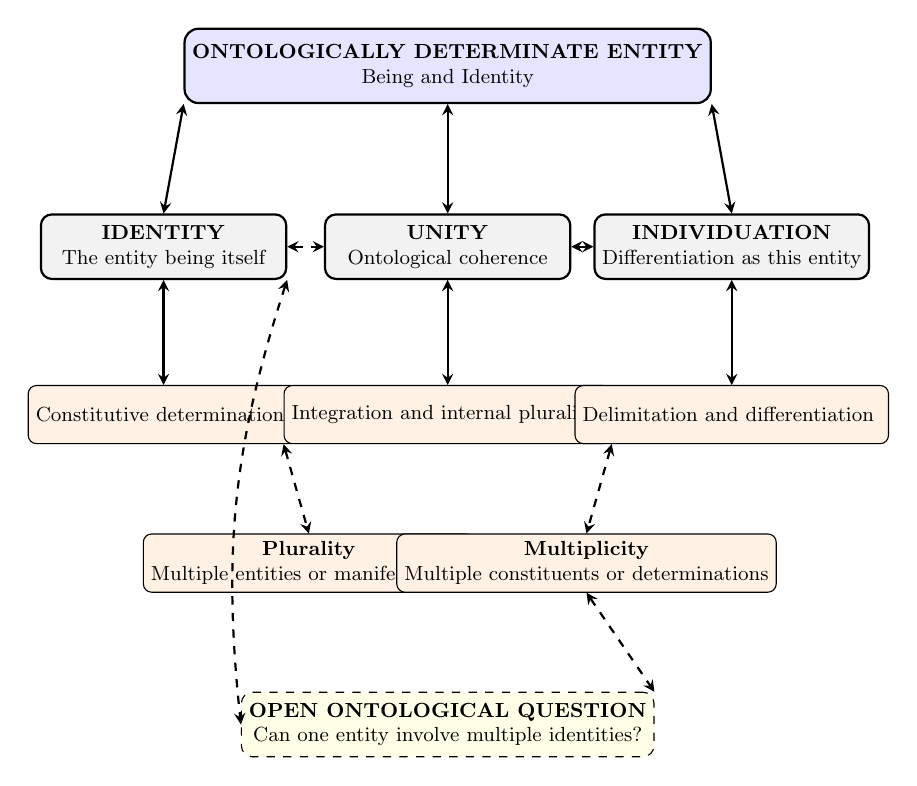
\begin{tikzpicture}[
        scale=0.82,
        transform shape,
        every node/.style={font=\small},
        core/.style={
            rectangle,
            rounded corners=5pt,
            draw=black,
            thick,
            minimum width=4.3cm,
            minimum height=1.15cm,
            align=center,
            fill=blue!10
        },
        concept/.style={
            rectangle,
            rounded corners=4pt,
            draw=black,
            thick,
            minimum width=3.8cm,
            minimum height=1cm,
            align=center,
            fill=gray!10
        },
        dimension/.style={
            rectangle,
            rounded corners=3pt,
            draw=black,
            minimum width=3.5cm,
            minimum height=0.9cm,
            align=center,
            fill=orange!10
        },
        openquestion/.style={
            rectangle,
            rounded corners=4pt,
            draw=black,
            dashed,
            minimum width=4.8cm,
            minimum height=1cm,
            align=center,
            fill=yellow!10
        },
        relation/.style={
            <->,
            thick,
            >=stealth
        },
        analytical/.style={
            <->,
            dashed,
            thick,
            >=stealth
        }
    ]

    % Central ontological entity
    \node[core] (entity) at (0,0) {
        \textbf{ONTOLOGICALLY DETERMINATE ENTITY}\\
        Being and Identity
    };

    % Three analytically distinct dimensions
    \node[concept] (identity) at (-4.4,-2.8) {
        \textbf{IDENTITY}\\
        The entity being itself
    };

    \node[concept] (unity) at (0,-2.8) {
        \textbf{UNITY}\\
        Ontological coherence
    };

    \node[concept] (individuation) at (4.4,-2.8) {
        \textbf{INDIVIDUATION}\\
        Differentiation as this entity
    };

    % Dimensions associated with each concept
    \node[dimension] (constitutive) at (-4.4,-5.4) {
        Constitutive determination
    };

    \node[dimension] (coherence) at (0,-5.4) {
        Integration and internal plurality
    };

    \node[dimension] (distinction) at (4.4,-5.4) {
        Delimitation and differentiation
    };

    % Plurality and multiplicity
    \node[dimension] (plurality) at (-2.15,-7.7) {
        \textbf{Plurality}\\
        Multiple entities or manifestations
    };

    \node[dimension] (multiplicity) at (2.15,-7.7) {
        \textbf{Multiplicity}\\
        Multiple constituents or determinations
    };

    % Open ontological question
    \node[openquestion] (question) at (0,-10.2) {
        \textbf{OPEN ONTOLOGICAL QUESTION}\\
        Can one entity involve multiple identities?
    };

    % Relations between the entity and its dimensions
    \draw[relation] (entity.south west) -- (identity.north);
    \draw[relation] (entity.south) -- (unity.north);
    \draw[relation] (entity.south east) -- (individuation.north);

    % Analytical distinctions
    \draw[analytical] (identity.east) -- (unity.west);
    \draw[analytical] (unity.east) -- (individuation.west);

    % Relations to associated dimensions
    \draw[relation] (identity.south) -- (constitutive.north);
    \draw[relation] (unity.south) -- (coherence.north);
    \draw[relation] (individuation.south) -- (distinction.north);

    % Internal plurality and multiplicity
    \draw[analytical] (coherence.south west) -- (plurality.north);
    \draw[analytical] (coherence.south east) -- (multiplicity.north);

    % The open question is not presented as a settled conclusion
    \draw[analytical] (identity.south east) to[bend right=12]
        (question.west);

    \draw[analytical] (multiplicity.south) -- (question.north east);

    \end{tikzpicture}

    \caption{The Relations Among Identity, Unity, and Individuation: Their Distinct Ontological Dimensions and the Open Question of Multiple Identities Within One Entity}
    \label{fig:identity-unity-and-individuation}
\end{figure}


The figure should be interpreted
as a conceptual representation rather
than as a causal, temporal, or hierarchical
sequence. It does not establish that
identity produces unity, that unity
produces individuation, or that
individuation is temporally subsequent
to identity.

It also preserves the open question
of whether one individual existent
may involve multiple identities.

\subsection{The Limits of an Ontology of Individuation}

The analysis establishes several
constraints for any subsequent
account of individuation.

First, individuation cannot be reduced
to identity, although the two are
ontologically related.

Second, individuation cannot be
identified with unity or with the
aggregation of components.

Third, distinction and qualitative
uniqueness do not provide sufficient
explanations of individuality.

Fourth, no universal principle of
individuation should be assumed
without establishing its applicability
to different kinds of existents.

Fifth, material, structural, and
relational conditions may contribute
to individuation, but their respective
roles must be examined rather than
presumed.

Sixth, individuation does not
automatically resolve the problem
of numerical identity and persistence.

Finally, the possibility of multiple
identities within one individual
existent remains open.

These constraints establish the
conceptual ground for a more precise
analysis of numerical identity and
the conditions under which an
individual remains the same existent.

\subsection{Concluding Formulation}

Individuation is the ontological
problem of how an existent is
constituted as a distinct individual
existent.

It is related to identity because
the individual is the existent whose
determinate character is under
consideration. It is related to unity
because an individual may constitute
a unity, including a unity involving
internal plurality. It is related to
distinction because individuation
concerns the constitution of an
existent as distinct.

Nevertheless, individuation cannot
be reduced to any of these concepts.

The central principle established
in this section is therefore:

\begin{quote}
Individuation concerns the ontological
constitution of an existent as an
individual. It is related to identity,
unity, and distinction, but cannot
be exhaustively explained through
any one of them.
\end{quote}

This principle establishes the basis
for examining numerical identity:
whether an individuated existent
remains one and the same existent
across different conditions and
transformations.



% =============================================================================
% SECTION 07
% IDENTITY AND NUMERICAL IDENTITY
% =============================================================================


\section{Identity and Numerical Identity}
\label{sec:identity-and-numerical-identity}

\subsection{The Ontological Problem of Numerical Identity}

Numerical identity concerns whether an existent considered
under different conditions is one and the same existent.

It must be distinguished from the broader ontological
problem of identity. Identity concerns the determinate
character through which an existent is the existent that
it is. Numerical identity concerns the sameness of an
individual existent across different conditions, states,
or moments of its existence.

The distinction is fundamental.

An account of what constitutes the identity of an existent
does not automatically resolve every question concerning
whether that existent remains numerically the same through
change. Conversely, establishing that an existent is
numerically the same across different conditions does
not provide an exhaustive account of its ontological
identity.

Numerical identity is therefore a specific problem within
the broader ontology of identity. It concerns the sameness
of an individual existent across a relevant comparison,
rather than the total constitution of its identity.

The problem is ontological rather than merely linguistic
or descriptive. The sameness of an existent cannot be
identified with the sameness of the expressions, properties,
or representations through which it may be characterized.

The central question is consequently whether the existent
under consideration remains one and the same existent
across the relevant conditions, and what ontological
conditions are involved in that sameness.

\subsection{Numerical Identity and Qualitative Identity}

A fundamental distinction must be established between
numerical identity and qualitative identity.

Numerical identity concerns whether two references or
considerations concern one and the same existent.

Qualitative identity concerns the sameness of particular
characteristics, properties, or determinations.

Two numerically distinct existents may be qualitatively
indistinguishable with respect to a specified set of
determinations. Conversely, one and the same existent
may undergo qualitative changes while remaining
numerically identical.

These possibilities establish that qualitative sameness
is neither sufficient nor universally necessary for
numerical identity.

If numerical identity were defined through the complete
preservation of qualitative characteristics, every
qualitative change would necessarily imply the termination
of the original existent and the emergence of another.
Such a conclusion cannot be adopted without independently
establishing that the relevant qualities are constitutive
of numerical identity.

Likewise, two existents cannot be considered numerically
identical merely because they share the same qualitative
configuration or because no relevant qualitative
difference has been established.

Qualitative similarity and numerical sameness therefore
belong to different analytical dimensions.

The numerical identity of an existent cannot be reduced
to qualitative resemblance, the coincidence of properties,
or the preservation of a descriptive configuration.

\subsection{Numerical Identity and Individuation}

Numerical identity is closely related to individuation,
but the two concepts address different ontological
questions.

Individuation concerns the ontological constitution
of an existent as an individual. Numerical identity
concerns whether that individual is one and the same
existent across different conditions.

Individuation therefore concerns the constitution
of individuality, whereas numerical identity concerns
the sameness of the individuated existent across
a relevant comparison.

The distinction is important because the constitution
of an existent as an individual under one condition
does not, by itself, resolve whether that individual
continues to exist as the same individual under
subsequent transformations.

An existent may be individuated while questions
concerning its numerical identity remain unresolved.

Conversely, the problem of numerical identity cannot
be adequately formulated without specifying the
individual existent whose sameness is at issue.

The two concepts are consequently mutually relevant
but analytically distinct. Individuation establishes
the problem of the constitution of an individual;
numerical identity establishes the problem of the
sameness of that individual across different conditions.

\subsection{Numerical Identity and Non-Identity}

Numerical identity can be expressed through the
distinction between an existent and any other existent.

If an existent A is numerically identical with an
existent B, A and B are not two distinct existents.
They are one and the same existent considered under
different references or conditions.

If A and B are numerically distinct, they are not
one and the same existent, even if they share
qualitative characteristics or structural configurations.

This distinction must not be confused with differences
between descriptions.

Different descriptions may concern one and the same
existent. Conversely, identical descriptions do not,
by themselves, establish that the existents to which
they are applied are numerically identical.

The ontological question concerns the existent itself,
not merely the expressions or descriptions through
which it is characterized.

Numerical identity therefore cannot be established
exclusively through linguistic equivalence, descriptive
consistency, or the coincidence of predicates.

It concerns the sameness of the existent across
the relevant comparison.

The distinction between numerical identity and
non-identity must also be preserved without assuming
that every difference between determinations constitutes
a difference between individuals.

\subsection{Numerical Identity and Change}

The relation between numerical identity and change
is one of the central problems in the ontology
of identity.

An existent may undergo changes in its properties,
states, relations, material constitution, or structural
organization. The occurrence of such changes does
not automatically establish that the existent has
become numerically different from itself.

However, the possibility of numerical identity
through change does not imply that every possible
transformation is compatible with the continued
existence of the same individual.

The relevant question concerns the ontological
significance of the transformation: which changes
are compatible with the continued numerical identity
of an existent, and which may affect the conditions
under which that existent continues to be the same
individual?

This question cannot be answered by treating all
determinations as equally significant.

Some changes may concern determinations that are
not constitutive of the numerical identity of
the existent. Other changes may affect its
constitutive organization or the conditions
through which it exists as the individual that
it is.

At least three possibilities must therefore
be distinguished:

\begin{itemize}
    \item A change in a determination that does
    not necessarily affect numerical identity.

    \item A change in a potentially constitutive
    determination that raises the question of
    whether numerical identity is preserved.

    \item A transformation that involves the
    termination of one individual and the
    emergence of another.
\end{itemize}

These possibilities must not be collapsed into
a single universal rule.

The ontological significance of a transformation
depends on the constitution of the existent and
the role of the determinations involved.

Numerical identity through change must therefore
be investigated in relation to the specific
conditions of the existent rather than through
an unrestricted assumption that either all
change preserves identity or every significant
change destroys it.

\subsection{Numerical Identity and Persistence}

Persistence concerns the continued existence
of an existent across different conditions.

Numerical identity is central to the problem
of persistence because persistence ordinarily
involves the continuation of one and the same
existent rather than the mere succession of
different existents.

Nevertheless, persistence and numerical identity
must not be treated as interchangeable without
qualification.

Persistence concerns the continuation of existence
across relevant conditions. Numerical identity
concerns whether the existent across those
conditions is one and the same individual.

This distinction makes it possible to examine
the conditions of continued existence without
assuming that every form of continuity establishes
numerical sameness.

An account of persistence must therefore address
the ontological basis of continuity, transformation,
and possible termination.

The present analysis does not assume that
persistence requires the preservation of every
property, determination, or material constituent.
Nor does it assume that the continued existence
of some material components is sufficient to
establish the numerical identity of the whole.

The relation between the persistence of components
and the persistence of the individual configuration
must be examined in its own right.

The conditions under which an individual persists
as numerically the same existent therefore remain
a distinct problem requiring further ontological
analysis.

\subsection{Material Continuity and Numerical Identity}

Material continuity provides one possible dimension
through which the persistence of an existent
may be examined.

An existent may retain some of its material
constituents while undergoing changes in other
aspects of its constitution. Conversely, its
material constitution may undergo substantial
replacement or transformation.

However, material continuity cannot automatically
be equated with numerical identity.

The persistence of particular material components
does not necessarily establish that the same
individual continues to exist. Conversely,
changes in material constitution do not necessarily
imply that the original individual has ceased
to exist.

The significance of material continuity depends
on the ontological nature of the existent and
the role of material constitution in its identity
and persistence.

For some existents, particular material conditions
may be constitutive of their continued numerical
identity. For others, material replacement or
transformation may be compatible with the
persistence of the same individual.

These possibilities cannot be resolved through
a universal assumption about the necessity
or sufficiency of material continuity.

Material continuity is therefore a potentially
significant condition in the analysis of numerical
identity, but it is neither an exhaustive definition
nor an independently sufficient criterion
of numerical sameness.

\subsection{Structural Continuity and Numerical Identity}

Structural continuity provides another dimension
of the problem of numerical identity.

An existent may preserve certain organizational
relations while its components, properties,
or other determinations undergo change.

Such continuity may be relevant to persistence,
particularly where structural organization
contributes significantly to the ontological
constitution of the existent.

Nevertheless, structural continuity cannot
automatically be treated as sufficient for
numerical identity.

Two numerically distinct existents may instantiate
the same structural organization. Conversely,
an individual may undergo structural modifications
without necessarily becoming a numerically
different existent.

The relevant question is whether the structure
under consideration is constitutive of the
individual's identity and whether its alteration
affects the conditions under which that individual
continues to exist.

Structural continuity must therefore be distinguished
from the mere repetition or preservation of
a structural pattern.

A pattern may persist across different existents
without establishing their numerical identity.
Likewise, the modification of a pattern does
not by itself establish the termination of
the individual in which it occurs.

Structural continuity is consequently a potentially
relevant condition of numerical persistence,
but its constitutive significance must be
established in relation to the existent concerned.

\subsection{Relational Continuity and Numerical Identity}

Relational continuity may also contribute
to the examination of numerical identity.

An existent may participate in relations that
persist across different conditions. Some of
these relations may be relevant to its continued
existence as the same individual.

However, the persistence of a relation does
not necessarily establish the persistence
of the individual involved.

A relation may continue to obtain even when
one of the existents participating in it has
been replaced by another. Conversely, the
alteration or termination of a particular
relation does not necessarily imply the
termination of numerical identity.

Relational continuity must therefore be
distinguished from numerical identity itself.

The ontological role of relations must be
examined in relation to the specific existent
and the conditions under which its individuality
and identity are maintained.

In particular, the persistence of a relational
position cannot be treated as an independently
sufficient criterion of numerical sameness.

Likewise, a change in relational conditions
cannot be assumed to produce a new individual
without establishing the constitutive significance
of the relations involved.

Relational continuity is therefore recognized
as a possible condition of numerical persistence,
not as a universal explanation of it.

\subsection{Numerical Identity and Invariance}

Numerical identity is related to the problem
of invariance, but the two concepts must not
be conflated.

Invariance concerns the preservation of a
specified feature, relation, or configuration
under a particular class of transformations.

Numerical identity concerns whether the existent
before and after a transformation is one and
the same existent.

An invariant may provide a basis for investigating
the preservation of identity. However, the
existence of an invariant does not, by itself,
establish numerical identity.

A structural pattern may remain invariant
across different individuals. Conversely,
the numerical identity of an existent may
be preserved even when some of its properties,
relations, or configurations change.

The relation between invariance and numerical
identity therefore depends on the ontological
significance of the invariant under consideration.

A particular invariant may be constitutive
of numerical persistence in a specific kind
of existent. Yet this possibility must be
established independently rather than inferred
from invariance alone.

This distinction is especially important
because invariance has sometimes been used
as a general definition of identity.

The present ontology does not accept the
reduction of identity or numerical identity
to invariance without an independent
ontological justification.

Invariance may be relevant to the analysis
of identity preservation, but it cannot
be presumed to provide a universal criterion
of numerical sameness.

\subsection{Numerical Identity and Signature}

A signature may characterize an existent
through a configuration of identifying features
or determinations.

Such a configuration may be relevant to
the distinction of an existent from others
or to the examination of its different
states and manifestations.

However, a signature is not necessarily
identical to the numerical identity of
the existent.

Two distinct existents may possess
indistinguishable signatures within a
particular descriptive or structural
framework. Likewise, the signature of
one existent may change without necessarily
implying that the existent has been
replaced by another.

The relation between signature and
numerical identity must therefore be
examined without reducing the latter
to the former.

A signature may provide a configuration
through which an existent is characterized,
but its constitutive significance for
numerical persistence must be established
rather than presumed.

The possibility that a signature may
preserve, express, or characterize certain
dimensions of an existent's identity
does not establish that it exhausts
the ontological conditions of numerical
sameness.

The distinction between the existent,
its numerical identity, and its signature
must therefore remain explicit.

\subsection{Numerical Identity and the Problem of Replacement}

The problem of replacement concerns
the conditions under which an existent
ceases to be the same individual and
another existent takes its place.

Replacement must be distinguished
from ordinary change.

An alteration in properties, relations,
or material constituents does not
necessarily constitute replacement.
Conversely, the preservation of certain
features does not necessarily exclude it.

The distinction requires an account
of the conditions that are constitutive
of the continued existence of the
individual.

Several questions therefore arise:

\begin{itemize}
    \item Under what conditions does
    transformation remain compatible
    with the numerical identity of
    an existent?

    \item When does a transformation
    affect the constitution of an
    individual to such an extent that
    its numerical identity is no longer
    preserved?

    \item Can a new existent emerge
    through the material or structural
    transformation of a previous
    existent?

    \item What is the ontological relation
    between the termination of one
    individual and the emergence of
    another?

    \item Can the termination of an
    individual and the emergence of
    another involve continuity in some
    constitutive conditions without
    establishing numerical identity
    between them?
\end{itemize}

These questions cannot be answered
through the mere identification of
qualitative differences or the preservation
of selected characteristics.

The present analysis therefore distinguishes
transformation from replacement while
leaving the specific conditions of
replacement open to further investigation.

In particular, the continuation of
some material, structural, or relational
conditions across a transformation
must not be confused with the numerical
identity of the individual before
and after that transformation.

\subsection{Numerical Identity and the Independence of Ontological Sameness}

Numerical identity belongs to the
ontological constitution and continuity
of the existent. It is not created
or eliminated by changes in the
descriptions or representations
through which an existent is characterized.

An existent may be characterized
under different descriptions without
thereby becoming a different existent.
Likewise, the absence of a description
or the omission of a particular
determination does not establish
the absence of numerical identity.

The distinction is important because
the ontological sameness of an existent
must not be confused with the identity
or difference of its descriptions.

Different descriptive configurations
may concern one and the same existent.
Conversely, the repetition of a
description or configuration does
not establish that two considerations
concern one and the same individual.

The present analysis therefore
treats numerical identity as independent
of descriptive equivalence, representational
continuity, and designation.

The issue is not how sameness is
established through a description,
but what ontological conditions
make an existent numerically the
same existent across different
conditions.

\subsection{The Relation Between Identity and Numerical Identity}

The analysis establishes a necessary
distinction between identity in its
broader ontological sense and
numerical identity as a specific
problem concerning the sameness
of an individual across different
conditions.

Identity concerns the determinate
character of an existent.

Numerical identity concerns whether
the existent considered under
different conditions is one and
the same individual.

The two concepts are related because
numerical identity concerns the
sameness of an existent whose
identity is under consideration.
Nevertheless, numerical identity
does not exhaust the broader
ontological constitution of identity.

Nor can the preservation of numerical
identity be inferred merely from
the persistence of qualitative
characteristics, material constituents,
structural patterns, relations,
invariants, or signatures.

Each of these conditions may be
relevant to the analysis of numerical
sameness, but its ontological role
must be examined independently.

The broader identity of an existent
and the numerical sameness of that
existent must therefore remain
distinct but related dimensions
of the ontology of identity.

\subsection{The Limits of an Ontology of Numerical Identity}

The preceding analysis establishes
several constraints for any subsequent
account of numerical identity.

First, numerical identity cannot
be reduced to the broader ontological
identity of an existent, although
the two are inseparable in the
examination of an individual existent.

Second, numerical identity cannot
be reduced to qualitative sameness
or the coincidence of properties.

Third, individuation and numerical
identity address different questions:
the constitution of an individual
and the sameness of that individual
across different conditions.

Fourth, change does not necessarily
terminate numerical identity, but
not every transformation can be
assumed to preserve it.

Fifth, material, structural, and
relational continuity may contribute
to numerical persistence, but none
can be assumed to constitute a
universal and sufficient criterion.

Sixth, invariance may be relevant
to identity preservation without
being identical to numerical identity.

Seventh, a signature may characterize
an existent without necessarily
exhausting the ontological conditions
of its numerical sameness.

Finally, transformation, replacement,
and the emergence of another existent
must be distinguished through an
examination of their constitutive
conditions rather than through
qualitative difference alone.

These constraints establish the
conceptual basis for examining
signature as a further dimension
of the ontology of identity.

\subsection{Concluding Formulation}

Numerical identity concerns whether
an existent considered under different
conditions is one and the same
existent.

It is a specific dimension of the
broader ontology of identity and
must be distinguished from qualitative
similarity, descriptive sameness,
material continuity, structural
continuity, relational continuity,
invariance, and signature.

These conditions may contribute
to the investigation of numerical
identity, but none can be assumed
to provide a universal and exhaustive
criterion of numerical sameness.

The central principle established
in this section is therefore:

\begin{quote}
Numerical identity concerns the
sameness of an individual existent
across different conditions. It is
a specific dimension of the broader
ontology of identity and cannot
be reduced to the preservation
of qualitative features, material
constituents, structural patterns,
relations, invariants, or descriptive
signatures. Its ontological conditions
must be examined in relation to
the constitution and persistence
of the individual existent concerned.
\end{quote}

This principle establishes the
basis for examining identity and
signature: the relation between
the ontological identity of an
existent and the configuration
through which its determinations
may be characterized.



% =============================================================================
% SECTION 08
% IDENTITY AND SIGNATURE
% =============================================================================

% =============================================================================
% Project : THE_PHILOSOPHY_OF_VIABILITY
% Book    : Book I — Ontology of Viability
% Book ID : VS.B01
%
% File    : 2_MAINMATTER/PART_I_IDENTITY/chapter_01_identity/sections/section_08_identity_and_signature.tex
%
% Section / Chapter:
%   Identity and Signature — Chapter 01: Identity
%
% Purpose :
%   To examine the relation between ontological identity and signature,
%   distinguish signature from determination, invariance, numerical identity,
%   individuation, and manifestation, and clarify the unresolved ontological
%   status of signature.
%
% =============================================================================

\section{Identity and Signature}
\label{sec:identity-and-signature}

\subsection{The Ontological Problem of Signature}

The relation between identity and signature raises a distinct
problem within the ontology of identity: whether an organized
configuration of determinations can characterize an existent
without thereby constituting, or exhausting, its identity.

An existent may involve multiple determinations and relations
that form an organized configuration. Some of these
determinations may be materially, structurally, or relationally
connected. Their configuration may provide a significant basis
for characterizing the existent in a particular respect. The
term \emph{signature} will be used for such an organized
configuration when considered in its characterizing role.

This use of the term does not yet settle the ontological status
of signature. In particular, it does not determine whether a
signature is merely an analytical configuration of actual
determinations, whether it corresponds to a distinct
ontological organization, or whether its status differs across
different kinds of existents.

The central question is therefore not simply whether a
signature can characterize an existent. It is whether the
characterizing role of a signature warrants identifying it
with the existent's identity, or assigning it a constitutive
role in that identity.

The distinction between identity and signature must be
maintained while these possibilities are examined.

Identity concerns what makes an existent the existent that
it is, without presupposing that its identity is reducible
to any single determination or configuration. Signature,
by contrast, concerns an organized configuration of
determinations through which an existent may be characterized
in a particular respect.

The two are related because a signature may involve
determinations that are relevant to the constitution,
character, or differentiation of an existent. Their relation,
however, does not establish their equivalence. Nor does the
fact that a signature characterizes an existent establish
that it provides a complete account of what that existent
is.

The present section therefore rejects the identification
of identity with signature while leaving open the more
specific question of whether, and under what conditions,
signature may participate in the ontological constitution
of identity.

\subsection{Identity Is Not Reducible to Signature}

Identity cannot be defined simply as the signature of an
existent.

Such a definition would make the identity of an existent
equivalent to a configuration of determinations selected
and organized as its signature. This would conflate the
ontological question of what the existent is with the
question of which determinations are brought together
to characterize it.

Several difficulties follow from this reduction.

First, a signature may be selective. It may include some
determinations while omitting others. If identity were
equivalent to signature, every omitted determination
would risk being treated as irrelevant to identity, even
where that determination might be ontologically
constitutive.

Second, signatures may be specified at different levels
of comprehensiveness or under different respects of
consideration. The same existent may consequently admit
different characterizations without there being sufficient
grounds to conclude that its identity has changed.

Third, determinations included in a signature may vary.
A change in one or more of them does not, by itself,
establish a change in numerical identity or in the
ontological constitution of the existent.

Fourth, the same configuration may characterize more
than one numerically distinct existent. A signature's
descriptive or structural distinctiveness within one
domain cannot therefore be assumed to provide a
universal criterion of individuation or numerical identity.

These difficulties do not show that signatures are
ontologically insignificant. They show that their
significance cannot be established by identifying them
with identity in advance.

A signature may be relevant to the constitution or
characterization of an existent. Whether that relevance
is constitutive, conditional, or merely characterizing
must be examined independently.

\subsection{Signature as an Organized Configuration}

A signature is not adequately understood as an arbitrary
list of properties. Its characterizing role depends on
the organization of the determinations involved.

A configuration may be organized through relations among
its determinations, through their arrangement, or through
the way in which they jointly characterize an existent.
The significance of the configuration may therefore
depend not only on which determinations are included,
but also on how they are related.

This does not imply that every signature possesses a
single organizing principle, that its components form
a unified whole, or that the organization is necessarily
intrinsic to the existent. These are further questions
that cannot be settled by the concept of signature alone.

Nor does the organization of a configuration establish
the ontological priority of its components. A determination
may be relevant to a signature without being ontologically
prior to the other determinations involved. Similarly,
the coherence of a configuration does not establish that
all its components are constitutive of identity.

The term signature thus identifies an organized
configuration considered in relation to the
characterization of an existent. It does not, by itself,
determine whether that organization constitutes an
ontological unity, an analytical grouping, or a
combination of both.

This distinction is necessary because an existent's
actual determinations and the configuration through
which some of them are considered are not automatically
the same thing. The determinations may belong to the
existent independently of whether they are grouped
together as a signature.

\subsection{Signature and Determination}

Signature and determination are related but non-equivalent.

Determination concerns the ontological condition through
which an existent is determinate. Signature concerns an
organized configuration involving determinations that
may be relevant to characterizing that existent.

A signature therefore does not constitute the totality
of an existent's determinations merely by bringing
some of them together. Its scope may be selective,
respect-dependent, or limited to a particular
configuration under consideration.

The omission of a determination from a signature does
not establish that the determination is absent from
the existent. Nor does it establish that the omitted
determination lacks ontological significance.

Conversely, the inclusion of a determination in a
signature does not establish that it is constitutive
of identity. Its inclusion establishes, at most, its
relevance to the configuration as specified. The
nature and extent of that relevance require separate
examination.

It is also necessary to distinguish the actual
determinations of an existent from the criteria through
which a signature is specified. A criterion of inclusion
may determine which features are considered together,
but it does not thereby determine which features
actually belong to the existent.

Signature is consequently neither an alternative
name for determination nor an exhaustive inventory
of determination. It is a configuration involving
determinations whose ontological relations and
significance cannot be inferred solely from their
participation in that configuration.

\subsection{The Ontological Status of Signature}

The distinction between identity and signature does
not, by itself, establish what kind of ontological
status signature possesses.

At least three possibilities must be distinguished.

First, a signature may be an analytical configuration:
a grouping of actual determinations considered together
for the purpose of characterizing an existent. On this
account, the configuration as a signature need not
constitute an additional ontological feature of the
existent, even though the determinations grouped
together are real.

Second, a signature may correspond to an organization
that belongs to the existent independently of its
description. In this case, the signature would not
merely collect determinations analytically; it would
also refer to an organization grounded in the existent
itself. Whether such an organization is constitutive
of identity would remain a further question.

Third, signature may have a conditional or domain-specific
ontological significance. Certain configurations may
participate in the constitution of particular kinds
of existents or in particular respects of their
identity, without signature having one universal
ontological function.

These possibilities should not be treated as an
exhaustive classification. They identify distinctions
that must be investigated before a general ontological
account of signature can be established.

In particular, the claim that a signature corresponds
to an actual organization does not entail that it
constitutes identity. Likewise, the claim that a
signature is analytically specified does not entail
that the determinations involved are merely descriptive
or lack ontological significance.

The ontological status of signature therefore remains
an open problem. The present analysis establishes
the non-equivalence of identity and signature, not
a definitive theory of signature's independent
ontological status.

\subsection{Signature and Invariance}

Signature may be related to invariance when some
determinations or relations within a configuration
remain preserved under specified transformations.

Invariance concerns the preservation of a specified
feature, relation, or configuration under a particular
class of transformations and with respect to a
specified domain. Signature concerns an organized
configuration of determinations considered in its
characterizing role.

A signature may contain invariant and variable
determinations. Its configuration may remain stable
under some transformations while changing under
others. Whether such changes affect the relevance
or organization of the signature depends on the
configuration and the transformations being considered.

Conversely, an invariant may be shared by multiple
numerically distinct existents. The preservation of
a feature under transformation therefore does not
necessarily distinguish one existent from another.

Neither the stability of a signature nor the
presence of invariants within it establishes that
the signature is identical to identity. Nor does
the absence of an identified invariant establish
that an existent lacks identity.

An earlier formulation of identity in terms of
invariance under allowable transformations cannot
therefore be transferred into the present account
without additional argument. Such a formulation
would require an independently justified account
of the relevant transformations, the domain of
application, and the respect in which preservation
is being considered.

Invariance may provide a condition for examining
the stability of particular signatures. It cannot
be assumed to provide a universal definition of
signature or identity.

\subsection{Signature and Numerical Identity}

Signature cannot be treated as a sufficient criterion
of numerical identity.

Two numerically distinct existents may possess
identical or indistinguishable signatures within
a specified domain and respect of comparison.
The sameness of their signatures therefore does
not establish that they are one and the same existent.

Conversely, the signature associated with one
existent may change as some of its determinations
or relations change. Such a change does not, by
itself, establish that the existent has ceased
to exist or that another existent has replaced it.

These possibilities show that the comparison of
signatures cannot independently settle the question
of numerical identity. Signature similarity does
not establish numerical identity, and signature
difference does not establish numerical non-identity.

This conclusion must be distinguished from the
question of persistence. Numerical identity concerns
whether different designations or considerations
refer to one and the same existent. Persistence
concerns whether an existent continues to exist
through relevant changes or conditions. A signature
may be relevant to an investigation of persistence,
but its stability is not, without further argument,
a sufficient criterion of persistence.

The ontological role of signature in the continuity
of an existent must therefore be investigated
without presupposing that the preservation of a
signature is either necessary or sufficient for
the persistence of that existent.

\subsection{Signature and Individuation}

Signature may characterize an individual existent
in relation to other existents. It does not thereby
explain how that existent is constituted as an
individual.

Individuation concerns the ontological constitution
of an existent as an individual. Signature concerns
an organized configuration of determinations through
which that individual may be characterized.

A signature may be distinctive within a particular
domain or respect of comparison. Such distinctiveness
may assist in differentiating an existent from
others under those conditions. It does not,
however, establish that the signature provides
the ontological ground of individuation.

Likewise, the absence of a unique signature does
not establish the absence of individuality. Two
numerically distinct individuals may share a
signature, or may be indistinguishable with respect
to the determinations included in a particular
configuration.

It follows that individuality must not be made
dependent upon the possession of an absolutely
unique signature. The possibility of shared
signatures does not eliminate numerical distinction,
just as a distinctive signature does not, by itself,
explain the constitution of an individual.

Signature may therefore contribute to the
characterization of individuality without being
identified with individuation or treated as its
universal ontological ground.

\subsection{Signature and Manifestation}

Signature and manifestation concern different
aspects of an existent.

Manifestation concerns the ways in which an existent
or its determinations become manifest under
particular ontological conditions. Signature
concerns an organized configuration of determinations
through which an existent may be characterized.

A particular manifestation may involve some
determinations associated with a signature without
exhausting that signature. Different manifestations
may also involve different subsets or arrangements
of determinations.

Such variation does not automatically establish
a change in identity. Nor does the fact that a
signature characterizes an existent establish
that the signature is itself a manifestation.

Three questions must therefore remain distinct:

\begin{itemize}
    \item What constitutes the ontological identity
    of an existent?

    \item Which organized configuration of
    determinations characterizes the existent
    in a specified respect?

    \item Under what ontological conditions do
    particular determinations become manifest?
\end{itemize}

These questions may constrain one another, but
their answers cannot be presumed to coincide.

The relation between signature and manifestation
also remains open in a further respect: a signature
may be associated with multiple manifestations,
while a manifestation may involve determinations
that are not included in a particular signature.
The precise relation depends on the organization
and scope of the configuration under consideration.

The present analysis consequently rejects both
the reduction of identity to signature and the
reduction of signature to manifestation.

\subsection{The Possibility of Multiple Signatures}

The distinction between identity and signature
allows for the possibility that one existent may
be characterized through more than one signature.

Different configurations may organize different
determinations or relations, or characterize
different respects of the same existent. Their
differences need not imply that the existent
possesses multiple identities.

Nor should the possibility of multiple signatures
be taken to establish that all such configurations
are equally comprehensive or ontologically
equivalent. One configuration may include
determinations omitted from another; two
configurations may overlap; or they may concern
different domains and respects.

These possibilities require distinctions among
the relations that may hold between signatures.
Overlap does not entail identity of configurations.
Partial inclusion does not establish ontological
priority. Difference between configurations
does not, by itself, establish difference between
the identities of the existents they characterize.

The possibility of multiple signatures must also
be distinguished from the question of whether
one existent can involve multiple identities.
The former concerns the plurality of configurations
through which an existent may be characterized.
The latter concerns the ontological constitution
of identity itself.

The possibility of multiple signatures is therefore
compatible with leaving the multiplicity of identity
unresolved. It neither establishes nor excludes
that possibility.

\subsection{Signature, Description, and Ontological Reality}

The characterization of an existent through a
signature must not be confused with the production
of the existent or its determinations through
description.

An existent does not acquire its identity because
a signature has been specified for it. Its actual
determinations do not depend for their existence
upon whether they have been collected into a
configuration or represented in a description.

A description may select, order, and represent
determinations associated with an existent. The
resulting representation may be more or less
comprehensive, accurate, or adequate to the
configuration it purports to characterize. These
features concern the description and its relation
to what it describes; they do not establish that
the existent itself is constituted by the
description.

The distinction between an actual configuration
and its description is therefore essential.
A description of a signature is not identical
to the signature, if the latter corresponds to
an organization grounded in the existent. If
signature is instead used analytically for a
selected configuration, the description still
does not create the determinations it brings
together.

The absence of a complete description does not
establish the absence of identity, determination,
or an actual organization. Nor does the
specification of a complete description establish
that the identity of the existent has been
exhaustively accounted for.

This preserves the ontological independence
of the existent from its characterization while
leaving open the question of whether signature
refers to an organization that possesses an
ontological status beyond its analytical
specification.

\subsection{The Limits of Signature as an Account of Identity}

The analysis establishes several constraints
on the use of signature within an ontology
of identity.

First, signature is not synonymous with identity.
An organized configuration of determinations
cannot be assumed to exhaust what makes an
existent the existent that it is.

Second, signature is not identical to the totality
of an existent's determinations. A configuration
may be selective without implying that omitted
determinations are absent or ontologically
irrelevant.

Third, the inclusion of a determination in a
signature does not by itself establish that
the determination is constitutive of identity.
Its constitutive significance requires an
independent argument.

Fourth, the organization of a signature does
not establish that it constitutes an ontological
unity or possesses an independent ontological
status.

Fifth, signature must not be reduced to invariance.
A signature may include both variable and
invariant determinations, and an invariant may
be shared by distinct existents.

Sixth, the sameness or difference of signatures
does not independently establish numerical
identity or numerical non-identity.

Seventh, a distinctive signature does not
establish the ontological ground of individuation,
and the absence of a unique signature does
not eliminate individuality.

Eighth, a change in signature does not
automatically establish a change in identity,
the end of an existent, or its replacement.

Ninth, multiple signatures associated with
one existent do not, by themselves, imply
multiple identities.

Finally, neither the analytical specification
of a signature nor its descriptive usefulness
settles its ontological status.

These constraints do not render signature
superfluous. They establish the conditions
under which its significance can be examined
without conflating characterization with
ontological constitution.

Signature remains relevant as a way of
considering organized configurations of
determinations. Whether particular configurations
also participate in the constitution of identity
is a further question, to be settled through
specific ontological arguments rather than
through the concept of signature alone.

\subsection{Conceptual Structure of Identity and Signature}

The distinctions developed in this section
can be summarized by separating identity,
determination, signature, invariance, numerical
identity, individuation, manifestation, and
description according to the questions each
concept addresses.

The following table records these distinctions.
It is an analytical guide, not a final taxonomy
of independent ontological entities or domains.

% =============================================================================
% Project : THE_PHILOSOPHY_OF_VIABILITY
% Book    : Book I — Ontology of Viability
% Book ID : VS.B01
%
% File    : 4_ASSETS/tables/VS.B01.P01.C01.S08.SS15.P001.TL01.identity_signature_conceptual_distinctions.tex
%
% Section / Chapter:
%   Identity and Signature — Chapter 01: Identity
%
% Asset:
%   TL01 — Identity and Signature: Conceptual Distinctions
%
% Purpose :
%   To distinguish identity from signature and related concepts,
%   clarifying their different analytical functions and preventing
%   unsupported ontological reductions.
%
% =============================================================================

\begin{table}[htbp]
    \centering
    \caption{Conceptual Distinctions Between Identity and Signature}
    \label{tab:identity-signature-conceptual-distinctions}

    \small
    \renewcommand{\arraystretch}{1.35}

    \begin{tabular}{p{0.19\textwidth} p{0.35\textwidth} p{0.36\textwidth}}
        \hline
        \textbf{Concept}
        &
        \textbf{Central Concern}
        &
        \textbf{Distinction from Signature}
        \\
        \hline

        Identity
        &
        What makes an existent the existent that it is.
        &
        Cannot be reduced to an organized configuration of determinations.
        \\

        Determination
        &
        The ontological condition through which an existent is determinate.
        &
        Signature involves selected and organized determinations but is not identical to determination as such.
        \\

        Signature
        &
        An organized configuration of determinations through which an existent may be characterized in a particular respect.
        &
        Its ontological status and possible constitutive role require independent examination.
        \\

        Invariance
        &
        The preservation of a specified feature, relation, or configuration under particular transformations.
        &
        May concern the stability of some signature components but does not define signature or identity.
        \\

        Numerical Identity
        &
        Whether different designations or considerations refer to one and the same existent.
        &
        Neither identical nor reducible to the sameness of signatures.
        \\

        Individuation
        &
        The ontological constitution of an existent as an individual.
        &
        A distinctive signature may characterize an individual without establishing its ontological ground.
        \\

        Manifestation
        &
        The ways in which an existent or its determinations become manifest under particular ontological conditions.
        &
        A manifestation may involve some signature determinations without exhausting the signature.
        \\

        Description
        &
        The representation or articulation of an existent or a configuration of its determinations.
        &
        A description of a signature must not be confused with the actual determinations or organization it represents.
        \\

        \hline
    \end{tabular}

    \vspace{0.5em}

    \begin{minipage}{0.92\textwidth}
        \footnotesize
        \textit{Note:} This table distinguishes analytical functions
        and ontological questions. It does not establish that every
        listed concept corresponds to an independent ontological
        entity or that the ontological status of signature has been
        definitively settled.
    \end{minipage}
\end{table}

% =============================================================================
% END OF TABLE TL01
% =============================================================================

The following diagram represents the principal
relations and non-equivalences examined in
this section. It distinguishes the existent
and its determinations from the configuration
considered as a signature and from the
description through which that configuration
may be represented.

% =============================================================================
% Project : THE_PHILOSOPHY_OF_VIABILITY
% Book    : Book I — Ontology of Viability
% Book ID : VS.B01
%
% File    : 4_ASSETS/diagrams/VS.B01.P01.C01.S08.SS15.P001.DG01.identity_signature_conceptual_relations.tex
%
% Section / Chapter:
%   Identity and Signature — Chapter 01: Identity
%
% Asset:
%   DG01 — Identity and Signature: Conceptual Relations
%
% Purpose :
%   To represent the conceptual distinction between an existent,
%   its determinations, an organized configuration considered as
%   a signature, and the description through which that configuration
%   may be represented.
%
% Technical Requirements (preamble):
%   \usepackage{tikz}
%   \usetikzlibrary{arrows.meta, positioning}
%
% =============================================================================

\begin{figure}[htbp]
    \centering
    \hyphenpenalty=10000 \exhyphenpenalty=10000\relax  % no hyphenation inside diagram labels

    \begin{tikzpicture}[
        font=\small,
        node distance=0.9cm and 0.7cm,
        % --- base box ---
        box/.style={
            draw, rounded corners=3pt, align=center,
            text width=3.4cm, minimum height=1.6cm,
            inner sep=5pt, line width=0.7pt
        },
        % --- node roles ---
        onto/.style    ={box, fill=blue!8, draw=blue!55!black},
        analytic/.style={box, dashed, fill=gray!10, draw=black!60},
        % --- arrows ---
        directed/.style={-{Stealth[length=2.5mm]}, thick},
        assoc/.style   ={{Stealth[length=2.2mm]}-{Stealth[length=2.2mm]},
                         thick, dashed}
    ]

    % ---------------------------------------------------------------
    % Grid: three columns, centered on Determinations
    % ---------------------------------------------------------------
    \node[onto] (determinations) {
        \textbf{Determinations}\\[2pt]
        Actual determinations of the existent
    };
    \node[onto, left=of determinations] (identity) {
        \textbf{Identity}\\[2pt]
        What makes the existent the existent that it is
    };
    \node[onto, right=of determinations] (manifestation) {
        \textbf{Manifestation}\\[2pt]
        Manifestation of an existent or its determinations
    };
    \node[onto, above=of determinations] (existent) {
        \textbf{Existent}\\[2pt]
        Ontological actuality
    };

    % ---------------------------------------------------------------
    % Analytical column (below Determinations)
    % ---------------------------------------------------------------
    \node[analytic, below=of determinations] (signature) {
        \textbf{Signature}\\[2pt]
        Organized configuration of determinations
    };
    \node[analytic, below=of signature] (description) {
        \textbf{Description}\\[2pt]
        Representation or articulation of a signature
    };

    % Numerical Identity: same column as Identity, same row as Signature
    \node[onto] (numerical) at (identity |- signature) {
        \textbf{Numerical Identity}\\[2pt]
        Reference to one and the same existent
    };

    % ---------------------------------------------------------------
    % Relations
    % ---------------------------------------------------------------
    \draw[directed] (existent)        -- (determinations);
    \draw[directed] (determinations)  -- (signature);

    \draw[assoc] (existent.west) -| (identity.north);
    \draw[assoc] (determinations)     -- (manifestation);
    \draw[assoc] (signature)          -- (description);
    \draw[assoc] (identity)           -- (numerical);

    % ---------------------------------------------------------------
    % Legend (bottom right, in the empty cell)
    % ---------------------------------------------------------------
    \node[anchor=center, draw=black!30, rounded corners=2pt,
          text width=3.4cm, align=left, font=\scriptsize, inner sep=5pt]
        (legend) at (manifestation |- description) {
        \textbf{Legend}\\[3pt]
        \tikz[baseline=-0.5ex]\draw[rounded corners=1pt, thick, fill=blue!8,
            draw=blue!55!black] (0,-0.1) rectangle (0.5,0.1);\;
        ontological concept\\[2pt]
        \tikz[baseline=-0.5ex]\draw[rounded corners=1pt, thick, dashed,
            fill=gray!10, draw=black!60] (0,-0.1) rectangle (0.5,0.1);\;
        analytical notion\\[2pt]
        \tikz[baseline=-0.5ex]\draw[directed] (0,0) -- (0.5,0);\;
        directed relation\\[2pt]
        \tikz[baseline=-0.5ex]\draw[assoc] (0,0) -- (0.5,0);\;
        association
    };

    % ---------------------------------------------------------------
    % Explanatory note
    % ---------------------------------------------------------------
    \node[below=0.8cm of description, text width=11cm, align=center,
          font=\footnotesize\itshape] (note) {
        Conceptual associations do not establish equivalence,
        causal production, or ontological reduction.
        The constitutive status of signature remains open.
    };

    \end{tikzpicture}

    \caption{Conceptual Relations Between Identity, Determination,
    Signature, and Description}
    \label{fig:identity-signature-conceptual-relations}
\end{figure}

% =============================================================================
% END OF DIAGRAM DG01
% =============================================================================

The diagram is conceptual rather than causal,
temporal, or hierarchical. It does not imply
that identity produces signature, that signature
produces invariance, or that manifestation
follows from signature. Nor does it establish
that signature is an independent ontological
layer.

In particular, the distinction between an
existent's actual determinations, their
organization, and the analytical specification
of a signature must not be mistaken for a
settled account of the ontological status of
that organization. The diagram preserves
the questions that remain open rather than
resolving them through visual arrangement.

\subsection{Concluding Formulation}

Identity and signature are related but
non-equivalent.

Identity concerns what makes an existent
the existent that it is. Signature concerns
an organized configuration of determinations
through which an existent may be characterized
in a particular respect.

A signature may characterize determinations
that are relevant to an existent's constitution.
It may also correspond, in some cases, to an
organization grounded in the existent itself.
Neither possibility establishes that signature
is identical to identity or that it exhausts
the ontological constitution of the existent.

The central principle of this section is
therefore:

\begin{quote}
The signature of an existent is not identical
to its ontological identity. It is an organized
configuration of determinations through which
the existent may be characterized, and whose
ontological status and possible constitutive
role must be established independently.
\end{quote}

This principle preserves the distinction
between an existent, its identity, the
determinations associated with it, and the
configurations through which those
determinations may be considered.

It also leaves open a substantive ontological
question: whether signature is exclusively
a mode of analytical characterization or
whether particular signatures may correspond
to, or participate in, real organizations
within the constitution of existents.

The non-reducibility of identity to signature
does not settle that question. It establishes
the conceptual and ontological distinctions
that any adequate answer must respect.

% =============================================================================
% END OF SECTION 08 OF CHAPTER 01
% =============================================================================



% =============================================================================
% SECTION 09
% IDENTITY AND NON-REDUCTION
% =============================================================================


\section{Identity and Non-Reduction}
\label{sec:identity-and-non-reduction}

\subsection{The Ontological Problem of Reduction}

The preceding sections have examined identity in relation to being, determination, unity, distinction, individuation, numerical identity, and signature. These examinations have established that identity cannot be conceptually identified with any one of these dimensions without an additional ontological argument.

The present section draws together the implications of those distinctions and formulates a general constraint for the ontology of identity: the principle of non-reduction.

Reduction occurs when a particular ontological determination, relation, condition, or mode of manifestation is treated as a sufficient and exhaustive explanation of what an existent is in its identity. Such a reduction may take the form of identifying identity with existence, the aggregation of determinations, unity, difference, individuation, numerical sameness, invariance, signature, structure, composition, material constitution, relational position, or manifestation.

Each of these dimensions may be relevant to identity. Some may participate in its constitution, determination, continuity, or articulation. The problem arises when their relevance is taken to establish their equivalence with identity.

The principle of non-reduction therefore does not deny the ontological significance of these dimensions. It denies that their significance, by itself, establishes their sufficiency as definitions of identity.

\subsection{Being and Identity: Inseparability Without Reduction}

The relation between being and identity provides the fundamental case for understanding non-reduction.

Being and identity are ontologically inseparable, analytically distinguishable, and neither has ontological priority over the other.

An existent does not first exist as an identity-free actuality and subsequently acquire identity as an additional determination. Nor can identity replace being, as though the determinate character of an existent could be considered independently of its actuality.

Consequently, identity cannot be reduced to being, because such a reduction would eliminate the question of the determinate ontological character of what exists. Equally, being cannot be treated as an ontological ground from which identity is subsequently derived.

Their distinction is analytical rather than a division into independently existing components. It permits the examination of different aspects of one ontological actuality without introducing an ontological separation between them.

This relation establishes an important limit for every subsequent account of identity: conceptual distinction must not be confused with ontological independence.

\subsection{Non-Reduction Across Ontological Determinations}

The distinctions developed in this chapter can be brought together through several related principles.

First, identity cannot be exhausted by determination. Although every existent is ontologically determinate, the totality or aggregation of its determinations does not automatically explain its identity. Not every determination is necessarily constitutive, and the accumulation of determinations does not by itself explain the ontological organization through which they belong to a particular existent.

Second, identity cannot be exhausted by unity, structure, or composition. Unity concerns the condition of an existent as a unity, while structure and composition concern aspects of its organization and constitution. These dimensions may be relevant to identity, but neither an account of unity nor an inventory of constituents necessarily establishes the determinate identity of the existent.

Third, identity cannot be reduced to distinction, difference, or individuation. Difference may contribute to the determination of an existent in relation to others, while individuation concerns its constitution as a distinct individual. Neither the establishment of difference nor the explanation of individual constitution necessarily provides a complete account of what that individual is.

Fourth, identity cannot be exhausted by numerical identity. Numerical identity concerns the sameness of an individual existent across different conditions. It does not, by itself, explain the full ontological character of that existent.

Finally, identity cannot be identified with signature or invariance. An organized configuration of determinations may characterize an existent, and the persistence of certain features under specified transformations may reveal aspects of continuity. Nevertheless, neither a signature nor an invariant configuration can be assumed to exhaust identity.

These principles do not establish that determination, unity, structure, composition, difference, individuation, numerical identity, signature, or invariance are ontologically independent of identity. They establish only that their respective explanatory roles cannot be presumed to be equivalent to identity itself.

\subsection{Material, Relational, and Manifestational Conditions}

The same principle applies to material constitution, relational determination, and manifestation.

Material constitution may participate in the identity of an existent. In some cases, particular material conditions may be essential to what an existent is; in others, material transformation may occur without necessarily establishing the loss of identity. Neither universal material continuity nor universal material replaceability can be assumed.

Relational determinations may likewise contribute to identity. An existent may be constituted or determined partly through relations with other existents, structural arrangements, or particular conditions. However, relational dependence does not establish that identity is reducible to relational position alone.

Manifestation introduces a further dimension. The way an existent becomes actual or expressed within a particular ontological context may disclose or realize aspects of its determinate character. Yet a particular manifestation cannot automatically be treated as an exhaustive account of identity. Differences between manifestations do not, by themselves, establish differences in the identity of the existent.

These cases demonstrate that the rejection of reduction must not be confused with the rejection of constitutive participation. Material, relational, structural, and manifestational dimensions may be involved in identity without being conceptually interchangeable with it.

Their precise ontological roles remain matters for further investigation.

\subsection{Conceptual Distinction, Ontological Distinction, and Relational Determination}

The principle of non-reduction requires a careful distinction among three levels of analysis.

\begin{enumerate}
    \item \textbf{Conceptual distinction:} Two concepts may express different meanings or explanatory functions without thereby referring to independently existing entities.

    \item \textbf{Ontological distinction:} Two aspects, determinations, or entities may be distinct in being. Such a claim requires an ontological argument and cannot be inferred from conceptual difference alone.

    \item \textbf{Relational determination:} Distinct concepts or ontological aspects may be related through conditions of dependence, constitution, participation, or interaction.
\end{enumerate}

These levels must not be conflated.

The fact that identity and unity are conceptually distinguishable does not, by itself, establish that they are independently existing ontological entities. Likewise, the fact that two dimensions are ontologically distinct does not establish that they are unrelated. A relation of constitution or dependence may connect dimensions that remain distinguishable.

Non-reduction therefore operates first as a constraint against conceptual equivalence. Whether the concepts involved also correspond to distinct ontological determinations, and how they are related, must be established separately.

This distinction prevents two opposite errors: reducing identity to another concept merely because the two are related, and isolating identity from other determinations merely because the concepts are distinguishable.

\subsection{Non-Reduction and Ontological Explanation}

The principle of non-reduction does not provide a complete explanation of identity. Rather, it establishes conditions that an adequate explanation must respect.

An ontological account of identity must examine the roles played by the different dimensions of an existent without assuming in advance that any one of them is sufficient. It must also distinguish among different forms of ontological relevance.

A determination may be constitutive of identity in one case but contingent in another. A relation may be necessary under particular conditions without being universally necessary. A structural or material feature may contribute to the identity of a particular kind of existent without providing a general definition applicable to every existent.

Accordingly, the following questions must remain distinguishable:

\begin{itemize}
    \item Whether a dimension is related to identity.
    \item Whether it participates in the constitution or determination of identity.
    \item Whether it is necessary or sufficient under specified ontological conditions.
    \item Whether its relevance is universal or limited to particular kinds of existents.
    \item Whether its alteration affects identity, continuity, or numerical identity.
\end{itemize}

No answer to one of these questions automatically determines the answers to the others.

Non-reduction thus requires more than the preservation of conceptual distinctions. It requires that claims about constitution, dependence, necessity, sufficiency, and continuity be justified independently rather than inferred from conceptual association.

\subsection{The Question of Multiple Identities}

The non-reduction of identity also leaves open the possibility that one existent may involve more than one identity.

The distinctions developed in this chapter do not provide sufficient grounds for either affirming or rejecting this possibility. The unity of an existent does not necessarily establish that it possesses only one identity. Conversely, internal plurality, compositional complexity, or structural differentiation does not establish that it possesses several identities.

Nor can multiple signatures, material configurations, structural arrangements, or manifestations be treated as evidence of multiple identities without further argument.

The question requires a more precise account of the relation between identity, unity, individuation, and the ontological constitution of an existent. In particular, it remains necessary to determine whether distinct identity determinations could belong to one and the same existent without implying the existence of multiple individuals.

This possibility must therefore remain an open ontological problem. It cannot be resolved merely by extending the conceptual distinctions established in the present chapter.

\subsection{The Principle of Non-Reduction}

The argument of this section can be summarized in the following principle:

\begin{quote}
Identity is not conceptually equivalent to any single ontological determination, condition, relation, or mode of manifestation associated with an existent. Its relation to being, determination, unity, distinction, individuation, numerical identity, signature, invariance, structure, composition, material constitution, relational determination, and manifestation must be examined without presuming that any one of these dimensions exhausts its ontological character. Their possible constitutive, relational, or explanatory relevance remains open to investigation.
\end{quote}

This principle establishes neither the absolute independence of identity nor the ontological independence of every concept related to it. It preserves the distinction between conceptual non-equivalence and ontological separation.

Being and identity remain ontologically inseparable, while the other dimensions examined in this chapter may participate in the constitution, determination, continuity, or manifestation of an existent in ways that require further justification.

Non-reduction is therefore a constraint on ontological explanation rather than a substitute for one. It prevents a partial determination from being treated as a complete account while preserving the possibility of discovering the relations through which the identity of an existent is constituted.

The problem of identity must consequently be pursued through an account that maintains conceptual distinction and ontological relation together.

\subsection{Transition to the Scope and Limits of Identity}

Having established that identity cannot be exhausted by any single related ontological concept, the investigation must now clarify the scope of the claims made about identity.

Non-reduction establishes what cannot be presumed about the relation between identity and its associated dimensions. It does not, by itself, determine the full extent of identity, the conditions under which particular determinations are constitutive, or the limits of the present account.

The following section therefore examines the scope and limits of identity as an ontological concept. Its purpose is to clarify what the present investigation has established, what remains provisional, and which questions must be reserved for subsequent parts of the ontology of viability.



% =============================================================================
% SECTION 10
% SCOPE AND LIMITS OF IDENTITY
% =============================================================================

% =============================================================================
% Project : THE_PHILOSOPHY_OF_VIABILITY
% Book    : Book I — Ontology of Viability
% Book ID : VS.B01
%
% File    : 2_MAINMATTER/PART_I_IDENTITY/chapter_01_identity/sections/section_10_scope_and_limits_of_identity.tex
%
% Section / Chapter:
%   The Scope and Limits of Identity
%
% Purpose :
%   To delimit the ontological claims established in the chapter,
%   distinguish foundational commitments from argued conclusions
%   and provisional constructions, and identify the principal
%   unresolved problems concerning identity.
%
% =============================================================================

\section{The Scope and Limits of Identity}
\label{sec:scope-and-limits-of-identity}

\subsection{The Need to Define the Scope of Ontological Claims}

An ontological investigation must establish not only the
distinctions through which a problem can be examined, but also
the limits of the claims that those distinctions support.

Without an explicit account of scope, conclusions may be
extended beyond the conditions under which they have been
established. A conceptual distinction may be mistaken for an
ontological separation, a possible relation may be treated
as a necessary one, or a partial explanation may be presented
as a universal principle.

The preceding sections have developed a framework for
investigating identity through its relations to being,
determination, unity, distinction, individuation, numerical
identity, and signature. They have also established a
constraint against reducing identity to any one of these
dimensions.

These conclusions clarify the conceptual and ontological
questions that an investigation of identity must address.
They do not, however, constitute a complete account of every
condition under which identity is constituted, maintained,
transformed, or manifested.

The purpose of this section is therefore to delimit the
scope of the present account, clarify the status of its
principal claims, and distinguish what has been established
from what remains provisional or unresolved.

The limits identified here concern the extent of the
arguments developed in this chapter. They must not be
confused with limits imposed upon existence or with claims
about what can or cannot be established by subsequent
ontological inquiry.

\subsection{The Ontological Scope of Identity}

The subject of this chapter is the ontological character
of identity.

Its central question concerns what makes an existent the
existent that it is. This question concerns the existent
itself and does not depend upon an act through which it is
identified, classified, named, or described.

Identity is therefore not treated as a product of
identification or as a determination introduced merely
through an external act. Its ontological status belongs
to the existent rather than to an activity directed toward it.

Within this scope, the chapter has examined the following
relations and distinctions:

\begin{enumerate}
    \item The ontological relation between being and identity.
    \item The relation between identity and determination.
    \item The distinction between identity and unity.
    \item The relations among identity, distinction, and difference.
    \item The relation between identity and individuation.
    \item The distinction between identity and numerical identity.
    \item The relation between identity and signature.
    \item The non-reduction of identity to other related
    ontological dimensions.
\end{enumerate}

These examinations establish a conceptual framework for
the further investigation of identity. They do not establish
that every existent has the same constitutive conditions,
that every dimension examined is relevant in every case,
or that the relations identified operate uniformly across
all possible kinds of existents.

The scope of the chapter is thus general in its ontological
question, but limited in the extent of the constitutive
principles it has established.

\subsection{Identity and Identification}

An important boundary of the present investigation concerns
the distinction between identity and identification.

An existent does not acquire its identity because an act
of identification occurs. Nor does the absence of such an
act imply the absence of identity.

The ontological character of an existent is not constituted
by its being named, classified, distinguished, or recognized
by another existent. Such activities may concern an
existent, but they do not provide the ontological ground
of its identity.

This commitment does not require a theory of identification,
nor does it determine the conditions under which identity
may become accessible to another existent. Those questions
concern additional relations and processes that are not
the subject of the present chapter.

The distinction is more limited and more fundamental:
the identity of an existent must not be made ontologically
dependent upon the occurrence of an identifying activity.

Accordingly, the present account treats identity as an
ontological question independently of whether identification
takes place. This does not entail that every possible
relation between an existent and another existent is
irrelevant to identity. It excludes only the assumption
that an act of identification is itself the ground from
which identity derives.

\subsection{The Limits of a Universal Definition}

The analysis developed in this chapter does not establish
a single universal principle that exhaustively determines
identity in every possible existent.

A principle may explain a particular dimension of identity
without explaining its complete ontological character.
An account of individuation, for example, may address the
constitution of an existent as an individual. An account
of invariance may address the preservation of selected
features or relations under specified transformations.
Neither explanatory function, by itself, establishes
a universal definition of identity.

The same limitation applies to principles based exclusively
on material continuity, structural organization, relational
stability, numerical identity, or the preservation of
a signature.

The present investigation therefore does not claim that
any one of these principles provides a universally
necessary and sufficient criterion of identity.

This limitation must be interpreted carefully. The absence
of an established universal criterion does not imply that
identity has no ontological conditions, nor does it imply
that such conditions are arbitrary. It means that their
general form, necessity, sufficiency, and domain of
applicability have not been established by the arguments
developed in this chapter.

Whether a more comprehensive principle can be formulated
remains an open problem.

The possibility of a universal account must therefore
be distinguished from the claim that such an account has
already been established. The former remains available
for investigation; the latter would exceed the present
argument.

\subsection{The Limits of Claims Concerning Persistence and Transformation}

Identity raises the question of how an existent remains
the existent that it is under different conditions and
through transformation.

The distinctions developed in this chapter prevent change
from being treated as automatically equivalent to the
loss of identity. They do not, however, establish a
universal criterion by which every transformation can
be classified as compatible or incompatible with the
persistence of an existent.

Material, structural, relational, and other determinations
may change in different ways and with different consequences.
Their significance cannot be assumed to be identical
across all kinds of existents.

Accordingly, the following distinctions must be maintained:

\begin{enumerate}
    \item Change does not necessarily entail the loss
    of identity.

    \item The continuity of selected determinations
    does not necessarily establish the persistence
    of identity.

    \item The preservation of a structure, signature,
    or invariant does not, by itself, establish
    numerical identity.

    \item The alteration or replacement of constituents
    does not, by itself, establish the destruction
    of an existent.

    \item Numerical identity across different conditions
    does not provide a complete explanation of the
    ontological character of the existent.

    \item The persistence of an existent and the
    preservation of every determination associated
    with it are not equivalent claims.
\end{enumerate}

These distinctions do not determine which transformations
preserve identity or which conditions are necessary for
persistence. They prevent such determinations from being
inferred solely from the presence or absence of selected
features.

A more comprehensive account must examine the relations
among identity, transformation, continuity, discontinuity,
replacement, and numerical identity in relation to the
kinds of existents and conditions under consideration.

The present chapter establishes the need for this
investigation, not its final criteria.

\subsection{The Limits of Claims Concerning Multiple Identities}

The present chapter does not establish whether one
existent can involve more than one identity.

The unity of an existent does not necessarily demonstrate
that its identity is singular in every relevant
ontological sense. Conversely, internal plurality,
compositional complexity, or structural differentiation
does not establish the existence of multiple identities.

The existence of multiple signatures, configurations,
determinations, or manifestations likewise does not entail
the existence of multiple identities. Such multiplicity
may concern different aspects or conditions of one
existent rather than distinct identity determinations.

The question requires a more precise account of the
relations among identity, unity, individuation, and the
ontological constitution of an existent. In particular,
it remains necessary to determine whether distinct
identity determinations could belong to one and the same
existent without implying the existence of multiple
individuals.

This inquiry must distinguish the possible multiplicity
of identity determinations from the numerical multiplicity
of individuals. The former, if established, would not
automatically entail the latter.

Neither the universal singularity nor the possible
plurality of identity can therefore be asserted on the
basis of the distinctions established so far.

The question remains open for subsequent ontological
investigation.

\subsection{The Limits of Universality Across Domains of Existence}

The conceptual framework developed in this chapter is
intended to support a general ontological investigation.
Nevertheless, its applicability across different domains
of existence does not establish that all identity-related
conditions operate identically in every domain.

A general ontological concept may retain its conceptual
function while the determinations through which it is
constituted or manifested vary according to the nature
of the existent.

Material constitution, structural organization, and
relational determination, for example, may have different
forms or degrees of relevance in different domains.
Such variation does not necessarily imply that identity
itself has an entirely different meaning in each domain.

Conversely, conceptual uniformity does not establish
that the ontological conditions of identity are uniform
throughout existence.

The present chapter therefore establishes neither the
complete uniformity nor the fundamental heterogeneity
of identity across all domains. It provides a general
conceptual framework whose applicability to particular
domains requires further examination.

The investigation of different realms of being must
determine how identity relates to their particular
ontological conditions without presupposing either
universal uniformity or absolute discontinuity.

The term ``domain'' is used here to designate a scope
within which particular ontological conditions are
examined. Its use does not establish a definitive
classification or hierarchy of domains, nor does it
presuppose that the proposed organization of the ontology
of viability is exhaustive.

\subsection{The Limits of the Relationship Between Identity and Manifestation}

The relation between identity and manifestation remains
only partially determined within the present investigation.

The chapter has established that identity cannot be
reduced to manifestation and that a particular
manifestation cannot automatically be treated as an
exhaustive account of the identity of an existent.

This does not establish that manifestation is merely
external to identity, or that the identity of an existent
remains unaffected by every possible condition of
manifestation.

A manifestation may involve particular determinations
of an existent under conditions associated with a
specific ontological context or domain. Whether such
conditions participate in the constitution, realization,
or transformation of identity requires further analysis.

The present chapter does not determine the complete
ontological status of manifestation or expression, nor
does it establish the relations among the domains in
which manifestation occurs.

These matters must be examined in the broader
investigation of manifestation and the realms of being.
Their relationship to identity cannot be settled merely
by the conceptual distinctions established here.

\subsection{The Limits of the Present Conceptual Framework}

The distinctions developed in this chapter provide
necessary conceptual conditions for a more comprehensive
ontology of identity. They do not yet provide a complete
account of its constitutive principles.

Several questions remain unresolved:

\begin{enumerate}
    \item What are the necessary and sufficient ontological
    conditions of identity?

    \item Can a general principle of identity be established
    across different domains of existence?

    \item How can constitutive determinations be distinguished
    from non-constitutive determinations in a general
    ontological account?

    \item Under what conditions can identity persist
    through substantial transformation?

    \item What is the complete relationship between
    identity, individuation, and numerical identity?

    \item Can one existent involve multiple identities
    without implying multiple individuals?

    \item What is the precise ontological relationship
    between identity and manifestation?

    \item To what extent are structure, composition,
    material constitution, and relational determination
    constitutive of identity?
\end{enumerate}

These questions identify the limits of the present account.
Their unresolved status does not, by itself, constitute
a contradiction within the framework or provide evidence
against its foundational commitments.

An unresolved question must not be treated as an
established conclusion. Equally, the absence of a
demonstrated principle must not be interpreted as proof
that such a principle is impossible.

The distinction between what has been established and
what remains open is therefore essential to the continued
development of the ontology.

\subsection{The Status of the Claims Developed in This Chapter}

The claims developed in this chapter must be distinguished
according to their argumentative and justificatory status.
Not all claims have the same function, and not all possess
the same degree or kind of support.

The following commitments provide the foundational
orientation of the present investigation:

\begin{enumerate}
    \item Being and identity are ontologically inseparable
    and analytically distinguishable.

    \item Neither being nor identity has ontological
    priority over the other.

    \item Identity is not an additional property attached
    to an identity-free existent.

    \item The ontological status of identity does not
    depend upon an act of identification.
\end{enumerate}

These commitments define the starting orientation of
the chapter. Their foundational role must not be confused
with the claim that every implication of them has already
been demonstrated.

The following distinctions have been developed through
the conceptual and argumentative analysis of the chapter:

\begin{enumerate}
    \item Identity is not conceptually equivalent to
    determination, unity, distinction, individuation,
    numerical identity, or signature.

    \item Conceptual non-equivalence does not establish
    ontological separation.

    \item Non-reduction does not imply ontological isolation.

    \item No single related ontological dimension has
    been established as an exhaustive definition
    of identity.
\end{enumerate}

These are conclusions of the chapter's analysis. Their
scope is limited to the arguments supporting them and
does not extend automatically to every possible
ontological relation among the dimensions concerned.

The following matters remain provisional or require
further ontological justification:

\begin{enumerate}
    \item The precise constitutive roles of material,
    structural, and relational determinations.

    \item The conditions under which particular
    transformations preserve or alter identity.

    \item The applicability of general identity principles
    across different domains of existence.

    \item The precise relation between identity and
    manifestation.
\end{enumerate}

The following remain open ontological problems:

\begin{enumerate}
    \item Whether a universal principle of identity
    can be established.

    \item Whether one existent can involve multiple
    identities.

    \item What constitutes a complete account of the
    necessary and sufficient conditions of identity.

    \item How identity, individuation, continuity,
    and numerical identity are related in a
    comprehensive ontology.
\end{enumerate}

This classification is local to the present chapter.
It is not a replacement for the broader system of
epistemic and justificatory statuses adopted by the
project. In particular, foundational commitments,
stipulated or defined claims, argued or derived claims,
conditionally supported claims, provisional constructions,
hypotheses, and unresolved problems remain distinguishable
within that broader system.

The classification above identifies the principal
groups of claims relevant to the present chapter; it
does not assign every individual proposition a final
status within the complete ontology.

Nor is this classification intended to establish a
permanent boundary around the theory. It clarifies
the current status of its claims and allows subsequent
arguments to develop, qualify, or revise them without
confusing foundational commitments with unresolved
possibilities.

\subsection{Ontological Restraint and the Development of the Theory}

The limits established in this section concern the
extent of the ontological claims justified by the
present investigation. They are not limitations
imposed upon existence itself.

Ontological restraint requires that the scope of every
claim remain proportionate to the argument supporting it.

A conceptual distinction may be established without
resolving every ontological relation between the
concepts involved. A possible condition may be
identified without being affirmed as universally
necessary or actual. A provisional construction may
organize further inquiry without being treated as a
completed ontological foundation.

This restraint is not a suspension of ontological
inquiry. It is a condition for its systematic development.

It also requires that the absence of a demonstrated
explanation be distinguished from the absence of an
ontological relation. The fact that a constitutive
relation has not yet been established does not show
that no such relation exists. Likewise, identifying
a possible relation does not establish that it is
necessary, universal, or sufficient.

The ontology of viability must therefore preserve
the distinctions among foundational commitments,
stipulated or defined claims, argued or derived claims,
conditionally supported claims, provisional constructions,
hypotheses, and open problems throughout its subsequent
development.

Such distinctions allow the theory to develop without
prematurely universalizing partial results or treating
unresolved questions as though they had already been
answered.

\subsection{Concluding Formulation}

The scope of the present investigation is the
ontological character of identity as inseparable from
the being of an existent. Its limits concern the extent
to which the constitutive conditions, principles, and
relations of identity have been established by the
arguments developed in this chapter.

The argument of this chapter supports the following
formulation:

\begin{quote}
Identity is an ontological dimension inseparable from
the being of an existent, but its complete constitution
cannot be inferred from any single related determination,
condition, or relation. The distinctions developed in
this chapter provide the conceptual conditions for
investigating identity without prematurely asserting
a universal criterion, a complete theory of persistence,
the singularity or plurality of identities, or an
exhaustive account of the relationship between identity
and manifestation.
\end{quote}

The present account establishes a foundational framework
for the ontology of identity, not a complete theory of
every condition under which identity is constituted,
maintained, transformed, or manifested.

Its unresolved questions define the direction of further
ontological inquiry rather than a deficiency in the
reality being investigated.

The chapter can therefore conclude with a distinction
between the ontological problem itself and the limits
of its present formulation: the identity of an existent
is not exhausted by the concepts through which it has
been examined, while the relations among those concepts
remain necessary subjects of further investigation.

The subsequent synthesis must preserve both sides of
this commitment: the ontological inseparability of being
and identity, and the need to investigate identity
without reducing it to any single related determination.

% =============================================================================
% END OF SECTION 10 OF CHAPTER 01
% =============================================================================


% =============================================================================
% SECTION 11
% SYNTHESIS OF IDENTITY
% =============================================================================

% =============================================================================
% Project : THE_PHILOSOPHY_OF_VIABILITY
% Book    : Book I — Ontology of Viability
% Book ID : VS.B01
%
% File    : 2_MAINMATTER/PART_I_IDENTITY/chapter_01_identity/sections/section_11_synthesis_of_identity.tex
%
% Section / Chapter:
%   Synthesis of Identity
%
% Purpose :
%   To synthesize the ontological commitments and arguments
%   developed throughout Chapter 01, preserve the distinctions
%   established among identity and its related dimensions, and
%   identify the unresolved problems that guide subsequent inquiry.
%
% =============================================================================

\section{Synthesis of Identity}
\label{sec:synthesis-of-identity}

\subsection{The Need for an Ontological Synthesis}

The preceding sections have examined identity through a
series of distinctions necessary for establishing its
ontological status. Being, determination, unity, distinction,
individuation, numerical identity, and signature have each
been considered in relation to identity. The investigation
has also examined the limits of reducing identity to
invariance, structure, composition, material constitution,
relational determination, or manifestation.

These distinctions are not intended to fragment the
ontological problem into unrelated conceptual domains.
Their purpose is to prevent the premature identification
of identity with any single dimension of existence while
making it possible to investigate the relations through
which identity may be constituted and determined.

A synthesis is therefore required. It must preserve the
distinctions established throughout the chapter while
bringing their implications together within a coherent
ontological position.

The objective is not to introduce a new principle that
replaces the preceding analysis, nor to claim that every
constitutive condition of identity has already been
discovered. It is to identify the commitments that can
be maintained at the present stage of the investigation,
the conclusions supported by the chapter's arguments,
and the problems that remain unresolved.

The synthesis must consequently preserve two requirements:
identity must not be reduced to any single related
ontological dimension, and its relations to those
dimensions must not be dismissed merely because they
are conceptually distinguishable.

\subsection{Identity as an Ontological Dimension of Existence}

The central foundational commitment of this chapter is
that identity is ontologically inseparable from being.

An existent does not first exist as an identity-free
substrate and subsequently acquire an identity. Being
and identity are not successive conditions, nor are they
two independently existing components that must be
externally combined.

Their distinction is analytical rather than ontologically
separative.

Being concerns the actuality of an existent, while
identity concerns what makes that existent the existent
that it is. These formulations address distinguishable
ontological questions without dividing the existent
into independently actual components.

Neither dimension can be removed from the relation
without altering the meaning of the other. This
inseparability, however, does not establish their
conceptual equivalence or make either one an exhaustive
definition of the other.

Identity must consequently be understood neither as
an additional property attached to an already constituted
identity-free existent nor as a merely descriptive
designation imposed upon it.

This position establishes the ontological significance
of identity without claiming that its complete
constitution has already been explained.

\subsection{Identity and Determination}

The relation between identity and determination is
essential to understanding the determinate character
of an existent.

An existent cannot be adequately considered as though
it were wholly indeterminate. Its being involves
determinations through which it is constituted and
through which its particular ontological character
may be investigated.

Nevertheless, identity cannot be identified with
determination as such, nor can it be reduced to the
accumulation or enumeration of an existent's
determinations.

Not every determination necessarily contributes to
identity in the same manner. Some determinations may
participate in constitution, while others may be
contingent, relational, situational, or dependent upon
particular conditions.

The distinction between determination in general
and determinations that may be constitutive of identity
is therefore essential.

Identity is related to determination because the
ontological character of an existent cannot be
investigated without considering its determinate
conditions. Yet this relation does not establish
that identity is identical with the totality of those
conditions or that their enumeration provides an
exhaustive explanation of identity.

The precise roles of particular determinations,
including their necessity, sufficiency, and possible
constitutive relations, remain subjects for further
ontological investigation.

\subsection{Identity and Unity}

Identity and unity are related but non-equivalent.

Unity concerns the constitution of an existent as a
unity, whereas identity concerns what makes that
existent the existent that it is.

The unity of an existent does not necessarily eliminate
internal plurality, compositional complexity, or
structural differentiation. Conversely, the identity
of an existent does not, by itself, explain every
condition through which its unity is constituted.

Unity therefore cannot serve as an exhaustive
definition of identity.

Nor does the distinction between identity and unity
establish that they are ontologically independent.
Their relation may involve conditions of constitution,
dependence, or participation that require further
argument.

The question of whether one existent may involve
multiple identity determinations also remains distinct
from the question of how that existent constitutes
a unity. Neither question can be resolved merely
by assuming that unity entails singularity of identity
or that internal plurality entails multiplicity of
identities.

\subsection{Identity, Distinction, and Difference}

Identity, distinction, and difference address related
but distinguishable ontological questions.

Identity concerns what makes an existent the existent
that it is. Distinction concerns the grounds upon which
entities, aspects, or determinations are distinguishable.
Difference concerns the ways in which determinations
or existents are non-identical or dissimilar.

An existent is not adequately characterized merely
by establishing that it differs from another existent.
Its identity cannot be reduced to its position within
a system of differences.

Likewise, the distinction of an existent from another
does not, by itself, explain the ontological character
of the existent being distinguished.

Nevertheless, difference and distinction may participate
in the determination of an existent. Their significance
depends upon the particular ontological relations and
conditions involved.

The synthesis therefore preserves both the
non-equivalence of identity and difference and the
possibility that distinction and difference contribute
to the determination of identity.

\subsection{Identity, Individuation, and Numerical Identity}

The relationship between identity and individuation
concerns the constitution of an existent as an individual.

Individuation addresses how an existent is constituted
as an individual, but an account of individual
constitution does not necessarily explain the complete
ontological character of that individual.

Numerical identity introduces a further distinction.
It concerns whether what is considered under different
references, descriptions, or conditions is one and
the same existent.

This question is essential to the examination of
sameness across different conditions, but it does
not provide an exhaustive definition of identity
or a complete account of persistence.

The three concepts therefore address related but
distinguishable ontological problems:

\begin{enumerate}
    \item \textbf{Identity} concerns what makes an
    existent the existent that it is.

    \item \textbf{Individuation} concerns the
    ontological constitution of an existent as
    an individual.

    \item \textbf{Numerical identity} concerns whether
    what is considered under different references
    or conditions is one and the same existent.
\end{enumerate}

Their relationships must be examined together without
treating them as interchangeable.

In particular, the question of how an existent is
individuated must remain distinguishable from the
question of whether it persists as numerically the
same existent through transformation.

\subsection{Identity and Signature}

A signature may provide an organized configuration
of determinations, relations, or features through
which aspects of an existent can be characterized.

Such a configuration may be relevant to the examination
of identity, but it cannot automatically be identified
with identity itself.

The existence of a signature does not establish that
every ontological determination of an existent has
been captured by it. Nor does the possibility of
multiple signatures necessarily imply the existence
of multiple identities.

Likewise, the alteration of a signature does not,
by itself, establish the loss of numerical identity.
The relation between a signature and the constitution
of identity must be examined rather than assumed.

The distinction between identity and signature is
therefore essential to preventing a descriptive or
configurational account from being treated as an
exhaustive ontological account.

The precise ontological status of signature and its
possible role in the constitution, determination,
or characterization of identity remain subjects
for further investigation.

\subsection{The Non-Reduction of Identity}

The preceding distinctions converge upon a general
ontological constraint: identity cannot be reduced
to any single related concept or determination
examined in this chapter.

It cannot be exhausted by being, determination,
unity, distinction, difference, individuation,
numerical identity, or signature. Nor can it be
exhaustively defined through invariance, structure,
composition, material constitution, relational
position, or manifestation.

However, non-reduction does not imply that identity
is isolated from these dimensions.

Each may participate in the constitution,
determination, continuity, differentiation, or
manifestation of an existent. Their precise roles
must be established through appropriate ontological
arguments rather than assumed in advance.

The synthesis therefore requires two simultaneous
commitments:

\begin{enumerate}
    \item Identity must remain conceptually
    distinguishable from its related ontological
    dimensions.

    \item The possible ontological relations among
    identity and those dimensions must remain open
    to investigation.
\end{enumerate}

These commitments prevent both reductionism and
ontological isolation.

The first prevents the explanatory role of a
particular dimension from being treated as proof
of its equivalence with identity. The second
prevents conceptual distinction from being
mistaken for the absence of ontological relations.

Non-reduction thus provides a constraint for
investigating identity without prejudging the
specific relations through which its constitution
may be understood.

\subsection{Identity and the Problem of Persistence}

The ontological status of identity raises the
question of how an existent remains the existent
that it is under changing conditions.

The present chapter establishes that change does
not automatically entail the loss of identity.
It also establishes that the continuity of selected
features does not automatically demonstrate the
preservation of identity.

Neither material continuity, structural persistence,
relational stability, nor the invariance of selected
determinations has been established as a universally
sufficient criterion.

The relationship between identity and persistence
must therefore be investigated through the specific
ontological conditions of the existent under
consideration.

A comprehensive account must eventually explain
how identity relates to transformation without
assuming either that all change destroys identity
or that every transformation is compatible with
its persistence.

It must also distinguish the persistence of an
existent from the preservation of every determination
associated with it, and distinguish both from
the question of numerical identity.

These problems remain open for further development.
Their resolution belongs to a more comprehensive
investigation of continuity, transformation, and
the conditions under which an existent persists.

\subsection{Identity and the Possibility of Multiple Identities}

The distinctions established in this chapter also
leave open the question of whether one existent may
involve more than one identity.

Unity does not necessarily establish the singularity
of identity, and internal plurality does not
necessarily establish its multiplicity.

Likewise, the presence of multiple determinations,
signatures, structural configurations, relations,
or manifestations does not independently demonstrate
that multiple identities are involved.

The possibility of multiple identities within one
existent requires a more comprehensive account of
the relationships among identity, individuation,
unity, and numerical identity.

In particular, it remains necessary to determine
whether distinct identity determinations could
belong to one and the same existent without
entailing the existence of multiple individuals.

No universal conclusion concerning the singularity
or plurality of identity is established here.

This question remains an explicit open problem
within the ontology of viability.

\subsection{The Independence of Ontology from an Identifying Subject}

The account developed throughout this chapter
concerns the existent and its identity independently
of an identifying or knowing subject.

Identity is not constituted by being recognized,
described, classified, or represented. The
ontological determination of an existent does
not depend upon the occurrence of an act of
identification.

This commitment concerns the ontological status
of identity and does not establish a complete
theory of the relations through which identity
may become accessible to another existent.

The ontology developed here must establish the
conditions and relations of existence without
presupposing the standpoint, capacities, or
operations of a knowing subject.

Questions concerning how an existent becomes
known, how its determinations become accessible,
and how knowledge relates to its manifestations
belong to a distinct investigation. They cannot
be used to replace the ontological problem of
identity developed in this chapter.

The independence of identity from identification
therefore establishes a boundary between the
ontological constitution of an existent and
the activities through which that existent
may subsequently be identified or understood.

\subsection{A General Ontological Formulation of Identity}

The arguments of this chapter support the
following formulation:

\begin{quote}
Identity concerns what makes an existent the
existent that it is. It is ontologically
inseparable from being while remaining analytically
distinguishable from being and from the other
ontological dimensions related to the constitution,
determination, unity, distinction, individuation,
and manifestation of an existent. No single one
of these dimensions has been established as an
exhaustive account of identity, although several
may participate in its constitution or
determination under particular ontological
conditions.
\end{quote}

This formulation expresses the central commitment
of the chapter without identifying identity with
determination or claiming to provide a complete
account of every condition through which identity
is constituted or maintained.

It establishes identity as an irreducible
ontological problem whose relations to other
dimensions of existence must be examined
systematically.

The formulation is therefore a general statement
of the position developed in this chapter, not
a demonstration of the necessary and sufficient
conditions of identity in every possible existent.

\subsection{Established Commitments and Remaining Problems}

The synthesis makes it possible to distinguish
the principal commitments maintained throughout
this chapter from the conclusions supported by
its arguments and the problems that remain
unresolved.

The following constitute the foundational
orientation adopted in the present investigation:

\begin{enumerate}
    \item Being and identity are ontologically
    inseparable and analytically distinguishable.

    \item Neither being nor identity has
    ontological priority over the other.

    \item Identity is not an additional property
    attached to an identity-free existent.

    \item The ontological status of identity
    does not depend upon an act of identification.
\end{enumerate}

These commitments define the foundational
orientation of the chapter. Their adoption
must not be confused with the claim that every
possible implication of them has already been
demonstrated.

The following conclusions have been developed
through the conceptual and argumentative analysis:

\begin{enumerate}
    \item Identity is not conceptually equivalent
    to determination, unity, distinction,
    individuation, numerical identity, or signature.

    \item Conceptual non-equivalence does not
    establish ontological separation.

    \item Non-reduction does not imply
    ontological isolation.

    \item No single related ontological dimension
    has been established as an exhaustive
    definition of identity.

    \item The explanatory relevance of a
    determination does not, by itself, establish
    its constitutive necessity or sufficiency.
\end{enumerate}

The following matters remain provisional or
require further ontological justification:

\begin{enumerate}
    \item The precise constitutive roles of
    material, structural, and relational
    determinations.

    \item The conditions under which particular
    transformations preserve or alter identity.

    \item The applicability of general identity
    principles across different domains of existence.

    \item The precise relation between identity
    and manifestation.

    \item The possible role of signature in the
    constitution or determination of identity.
\end{enumerate}

The following remain open ontological problems:

\begin{enumerate}
    \item Whether a universal principle of identity
    can be established.

    \item Whether one existent can involve
    multiple identities.

    \item What constitutes a complete account
    of the necessary and sufficient conditions
    of identity.

    \item How identity, individuation, continuity,
    persistence, and numerical identity are
    related in a comprehensive ontology.

    \item Whether the constitutive conditions of
    identity vary across different domains of
    existence, and in what respects.
\end{enumerate}

These groups identify the principal status of
the claims relevant to the synthesis. They are
not intended to replace the broader system of
functional and justificatory classifications
adopted by the project.

In particular, foundational commitments,
stipulated or defined claims, argued or derived
claims, conditionally supported claims,
provisional constructions, hypotheses, and
unresolved problems remain distinguishable
within that broader system.

The classification presented here is a
chapter-level synthesis rather than a final
assignment of status to every proposition
within the ontology.

It also does not establish a permanent boundary
around the theory. Subsequent investigations
may develop, qualify, or revise particular
conclusions, provided that the distinction
between adopted commitments, supported claims,
and unresolved problems is preserved.

\subsection{The Role of Identity in the Ontology of Viability}

Identity constitutes an indispensable problem
for the broader ontology of viability because
any investigation of existence, determination,
transformation, continuity, and manifestation
must address what it means for an existent to
be the existent that it is.

Without examining identity, subsequent
investigations would leave insufficiently
clarified the ontological question concerning
the existent whose determinations, relations,
transformations, and manifestations are being
considered.

However, this does not establish identity as
an ontological principle that is prior to or
exhaustive of the other dimensions of existence.
Its importance lies in the problem it identifies
and the distinctions necessary for investigating
that problem.

The ontology of viability must therefore
investigate the relations between identity and
the broader organization of existence without
assuming that the distinctions established
here have already resolved every question
concerning those relations.

Identity provides an indispensable point of
reference for further ontological inquiry,
but it does not substitute for the investigation
of the other dimensions through which existence
may be constituted, determined, and manifested.

\subsection{Concluding Statement}

The synthesis of this chapter establishes
identity as an irreducible ontological dimension
inseparable from the being of an existent.

Its conceptual distinction from determination,
unity, difference, individuation, numerical
identity, signature, structure, composition,
material constitution, relations, and
manifestation does not imply isolation from
them. Rather, it makes possible a more precise
investigation of how these dimensions are
related without prematurely identifying one
with another.

The chapter has therefore established a
foundational orientation and a set of
conceptual and argumentative constraints
for an ontology of identity while preserving
the questions that require further argument.

The resulting position can be expressed
in its most concise form:

\begin{quote}
An existent is the existent that it is through
an identity ontologically inseparable from
its being. This identity cannot be reduced
to any single related determination, condition,
or relation, although its constitution and
continuity may involve multiple ontological
dimensions whose precise relations remain
subjects for further investigation.
\end{quote}

With this synthesis, the initial ontological
examination of identity reaches its conceptual
conclusion. This conclusion does not complete
the ontology of identity or settle every
question concerning its constitution,
persistence, or manifestation.

It establishes the position from which
subsequent ontological investigations can
proceed: identity is inseparable from being,
irreducible to any single related dimension,
and open to further examination through the
relations and conditions that may participate
in its constitution.

% =============================================================================
% END OF SECTION 11 OF CHAPTER 01
% =============================================================================


% =============================================================================
% CHAPTER CONCLUSION
% =============================================================================

\section*{Chapter Conclusion}
\addcontentsline{toc}{section}{Chapter Conclusion}

This chapter has established identity as a
foundational dimension of ontological actuality
and has examined its relation to several other
fundamental ontological concepts.

Its central commitment is the inseparability
of being and identity, together with their
analytical distinguishability and the absence
of ontological priority between them.

The investigations have also established that
identity cannot be exhaustively defined through
any single related determination or ontological
dimension. Determination, unity, distinction,
individuation, numerical identity, and signature
address different aspects of the problem, while
their possible constitutive and relational roles
require examination rather than presumption.

The resulting position is one of ontological
non-reduction without ontological isolation.
The distinction between identity and related
concepts does not establish their ontological
independence. Nor does their possible involvement
in the constitution of an existent justify
reducing identity to any one of them.

The chapter has deliberately left several
questions unresolved. These include the
necessary and sufficient conditions of identity,
the possibility of multiple identities associated
with one existent, the continuity of identity
through transformation, and the precise relation
between identity and manifestation.

Their resolution requires further ontological
investigation and cannot be obtained merely
from the distinctions established in this chapter.

The position reached can therefore be stated
in the following terms:

\begin{quote}
An existent is the existent that it is through
an ontological identity inseparable from its
being. This identity is not reducible to any
single related determination, although its
constitution, continuity, and manifestation
may involve multiple ontological dimensions
whose precise relations require further
investigation.
\end{quote}

Identity is thus established as a foundational
but non-exhaustive dimension of the Ontology
of Viability. Its investigation provides a
necessary starting point for examining the
other dimensions and domains of existence
without prematurely determining their complete
ontological organization.


% =============================================================================
% END OF CHAPTER 01
% =============================================================================